\chapter{弹性波波动方程反射走时反演}

\section{引言}
%尽管常规FWI在长偏移距,宽方位数据中有着令人满意的效果,但是在这种观测系统下,
目前FWI应用成功的案例中,主要利用了长偏移距透射波以及临界反射波等来更新速度模型的
中低波数分量。中深部的模型更新则主要集中在偏移响应对应的高波数部分。
在中深部区域,即使以目前大偏移距、宽方位的观测技术也难以保证有足够的透射波穿过。
如何利用现有数据准确反演中深部速度模型的中低波数成分是人们非常关心的课题。

反射波可以更好地照明深部结构。
受MBTT方法的启发,Xu et al
(2012)\cite{xu:2012}提出了反射波波形反演方法(RWI),
通过反射波来产生类似透射路径的信息来获得中低波数成分的更新。
RWI基于波动理论建立中深部背景模型的思路立即获得了广泛的关注(Wang et al., 2013\cite{Wang2013}; Wu and Alkhalifah, 2015; 
Zhou et al., 2015\cite{zhou:2015}; Guo and Alkhalifah, 2016\cite{Guo2016})。
它实质是通过最小平方偏移等手段获取“真振幅”的反射率,然后利用反偏移预测出反射波数据,并将它与观测数据的波形残差
反投影到Born波路径上进行背景速度更新。
%近期,Irabor and
%Warner(2016)\cite{Irabor2016}和Wang et
%al(2016)\cite{WangFangEtAl2016}在初始模型中加入高频扰动并通过上下形波分离来获取常规FWI中能够更新背景速度的梯度分量,实质上也利用了反射波波路径的信息。
%然而波形匹配并非是RWI中最合适的拟合方式。
尽管RWI的目的在于更新背景速度,
当初始模型偏离真值较远时,反射波波形匹配也会受到cycle-skipping影响。这时分频等多尺度策略会有助于避免cycle-skipping现象\cite{Wang2013}。此外,利用
走时信息构建目标函数也可以较好地避免上述问题。

在成像域利用反射波更新背景速度的方法由来已久,如射线层析\cite{Stork1992}。波动方程速度偏移分析(WEMVA)近年来也获得了长足的发展(
Sava and
Fomel(2006)\cite{SavaEtAl2006}; Yang and Sava(2011)\cite{YangEtAl2011}; Almomin and
Biondi(2012)\cite{Almomin2012}; Sun and Symes(2012)\cite{SunEtAl2012})。
WEMVA通常需要引入扩展成像条件,采用各类准则衡量成像残差,例如叠加能量最大(SI)\cite{ChaventEtAl1995}、微分相似优化(DSO)\cite{SymesEtAl1991}
和差异剩余偏移(DRM)\cite{SavaEtAl2004}等来实现背景模型的更新。
但WEMVA受困于昂贵的计算代价,尤其在三维问题中。
%针对反射走时,Luo et
%al(2016)\cite{Luo2016}用时间轴方向的扩展成像与Rytov近似结合,导出了全走时反演(FTI)方法,获得了不错的反演效果。该方法实质上也是一种成像域的反演方法。

为了克服振幅拟合有关的目标函数带来的非线性,本章采用与背景速度更加线性相关的
走时信息来构建目标函数。通过动态图像识别(DIW)技术来获取模拟与观测反射数据之间的时移量\cite{ma2013},提出了弹性波波动方程反射走时反演(EWERTI)方法。
相比互相关提取时移(空移)量的方式\cite{chi2015,Wang2015},DIW能更准确地获取局部的走时差异。
%Ma and
%Hale(2013)\cite{ma2013}采用动态图像识别(DIW)来获得模拟与观测反射数据之间的时移,从而导出了波动方程反射走时反演(WERTI)。Chi
%et al (2015)\cite{chi2015}和Wang et al
%(2015)\cite{Wang2015}采用互相关类的方法来获取时移(或空移)。
此外,弹性波走时反演中需要处理模式转换产生的虚假反射波路径的问题,即
需要根据对应的PP波与PS波波路径(假设P波震源)更新$V_p$与$V_s$模型。
文中将联合地面P/S分离+DIW获取不同波模式的走时残差,并通过空间波场模式解耦预条件梯度来降低非线性程度、压制参数耦合等。
在此基础上,设计出两步的反演流程来实现稳健的EWERTI方法。Sigsbee2A模型的数值实验将验证EWERTI方法的有效性。
%但尽管如此,RWI中的强非线性问题仍然存在,尤其是在使用波形匹配的目标函数时。
%虽然波形信息能提高反演精度,但是走时信息对模型的低波数成分扰动更敏感,二者之间具有更好的线性关系。
%因此我们使用走时残差的$L_2$范数
%作为目标函数,而走时信息则采用DIW获取。
%由于PP与PS走分别包含在在P波与S波地震记录中,因此还需要采用地面数据分离的方式
%分解出P或S波数据,才能保证准确获取PP和PS波走时信息。%本章中采用EWERTI的方式,通过两步法的策略建立$V_p$与$V_s$的背景模型。
%所以,采用走时反演来为常规FWI建立合适的含有长波长信息的初始
%%模型会更加稳健有效\cite[]{Ma2013, Chi2015, Luo2016}。然而在弹性介质中,这中思路会受到限制,
%因为弹性波场中存在复杂的模式转换,这就导致很难获得单一波模式的走时
%信息。
\section{弹性波波动方程反射走时反演}
利用拟合反射波来反演模型参数就需要预测出反射波数据,再与观测数据进行匹配。
弹性反射波的模拟通常采用偏移/反偏移的方式实现。
在EWERTI中,需要匹配反射波数据的走时信息,
并将走时残差反投影到反射波路径上更新背景速度模型。下面从弹性波方程出发导出EWERTI的梯度公式。
反演过程中,
同样假设在背景弹性介质($c_{ijkl}$)中有参数扰动$\delta c_{ijkl}$,则背景波场与扰动波场分别满足以下方程:
\begin{equation}
    \rho \frac{\partial u^2_i}{\partial t^2}  -
    \frac{\partial}{\partial x_j}\left[ 
        c_{ijkl}\frac{\partial u_{k}}{\partial
        x_l}\right]=f_i,
    \label{eq:WE_3} 
\end{equation}
和
\begin{equation}
    \rho \frac{\partial \delta u^2_i}{\partial t^2}  -
    \frac{\partial}{\partial x_j}\left[ 
        c_{ijkl}\frac{\partial \delta u_{k}}{\partial
        x_l}\right]=\frac{\partial}{\partial x_j}\left[\delta c_{ijkl}\frac{\partial u_{k}}{\partial x_l}\right],
    \label{eq:DeltaWE} 
\end{equation}
这里$\delta u_i$可以看作是用ERTM或其他方法获得的成像结果($\delta c_{ijkl}$)进行反偏移构建的反射波数据。
观测数据$\mathbf{d}^{o}$与模拟数据$\mathbf{d}^{c}$之间的走时残差需要达到最小,则目标函数写成:
\begin{equation}
	\left\{
		\begin{aligned}
			&\tau(\mathbf{x_r},t;\mathbf{x_s})=\mathop{\arg\min}_{\tau}
			\parallel\mathbf{d}^{c}(\mathbf{x}_r,t;\mathbf{x}_s)-\mathbf{d}^{o}(\mathbf{x}_r,t+\tau;\mathbf{x}_s)\parallel^2\\
    &E=\frac{1}{2}\int\tau^2(\mathbf{x_r},t;\mathbf{x_s})dtd\mathbf{x_r}d\mathbf{x_s},
		\end{aligned}
	\right.
    \label{eq:Objectivefunction} 
\end{equation}
其中走时残差$\tau(\mathbf{x_r},t;\mathbf{x_s})$可以通过DIW技术来获取。通过类似Ma and
Hale (2013)\cite{ma2013}的推导(见附录\ref{cha:AdjointForEWERTI}),本文导出了如下梯度公式:
\begin{equation}
    \frac{\partial E}{\partial c_{ijkl}}=-\int (\frac{\partial u_{i}}{\partial
    x_j}\frac{\partial \delta \psi_{k}}{\partial x_l}+\frac{\partial \delta u_{i}}{\partial
    x_j}\frac{\partial \psi_{k}}{\partial x_l}),
    \label{eq:GradientCijkl}
\end{equation}
其中,$\psi_i$和$\delta \psi_i$是共轭的背景波场和散射波场,满足:
\begin{equation}
    \rho \frac{\partial \psi^2_i}{\partial t^2}  -
    \frac{\partial}{\partial x_j}\left[ 
        c_{ijkl}\frac{\partial \psi_{k}}{\partial
        x_l}\right]=\tau(\mathbf{x_r},t;\mathbf{x_s})\frac{\dot{d}^o_i(\mathbf{x_r},t+\tau;\mathbf{x_s})}{h_i(\mathbf{x_r},t;\mathbf{x_s})},
    \label{eq:AdjointWE} 
\end{equation}
和
\begin{equation}
    \rho \frac{\partial \delta \psi^2_i}{\partial t^2}  -
    \frac{\partial}{\partial x_j}\left[ 
        c_{ijkl}\frac{\partial \delta \psi_{k}}{\partial 
        x_l}\right]=\frac{\partial}{\partial x_j}\left[\delta c_{ijkl}\frac{\partial
        \psi_{k}}{\partial x_l}\right], 
    \label{eq:AdjointDeltaWE} 
\end{equation}
式中$h_i(\mathbf{x_r},t;\mathbf{x_s})=(\dot{d}^o_i(\mathbf{x_r},t+\tau;\mathbf{x_s}))^2-\ddot{d}^o_i(\mathbf{x_r},t+\tau;\mathbf{x_s})
(d^c_i(\mathbf{x_r},t;\mathbf{x_s})-d^o_i(\mathbf{x_r},t+\tau;\mathbf{x_s}))$,而$\dot{d}$则代表$d$的时间导数。
需要注意的是,上式伴随源的分母中包含有地震记录的二阶导数,会导致除法的不稳定,这里采用时间方向的积分
$h^{'}_i(\mathbf{x_r};\mathbf{x_s})=\int h_i(\mathbf{x_r},t;\mathbf{x_s})dt$
来代替原有的分母项(付继有等,2015\cite{Fu2015})。
在方程\eqref{eq:GradientCijkl}的右端
,第一和第二项分别表示震源端和检波点端的反射波路径。可以通过链式法则导出P波与S波速度的梯度公式:
\begin{equation}
\begin{split}
    &\frac{\partial E}{\partial V_p}=2\rho V_p\frac{\partial E}{\partial
        c_{ijkl}}\delta_{ij}\delta_{kl}, \\
    &\frac{\partial E}{\partial V_s}=2\rho V_s\frac{\partial
    E}{\partial c_{ijkl}}(-2\delta_{ij}\delta_{kl}+\delta_{ik}\delta_{jl}+
    \delta_{il}\delta_{jk}).
\end{split}
    \label{eq:GradientVel}
\end{equation}

\section{弹性波反射波路径核函数}
反射波反演的关键是将预测的与观测的反射波之间的残差反投影到反射波路径上,从而实现对模型的更新。因此,反射波波路径的计算将是反演中
的核心任务。由于弹性波中存在各种模式转换,所以反射波波路径的复杂程度远大于声波中的情况。首先分析弹性波反射波路径的性态,并尝试通过
模式解耦克服反演中遇到的部分困难。
由附录\ref{cha:AdjointForEWERTI}推导可看出,不同的目标函数只影响共轭状态方程的伴随震源项,并不影响最终梯度的互相关方式。
因此分析弹性反射波波路径的核函数性态将有助于理解模式耦合引起的问题,从而为压制梯度中的假象并帮助设计新的反演策略提供理论依据。
\begin{figure}[!htb]
   \centering
   \subfloat[]{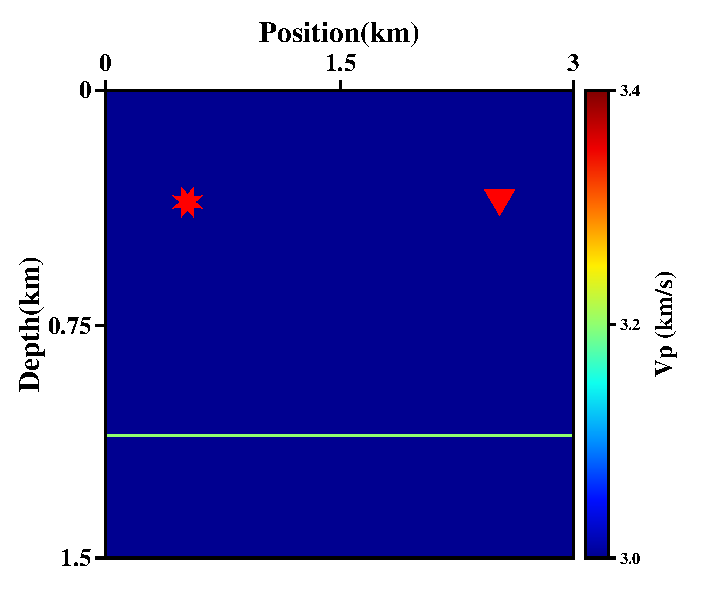
\includegraphics[width=0.50\textwidth]{Figure/chapter03/Kernel/1vp.pdf}}
   \subfloat[]{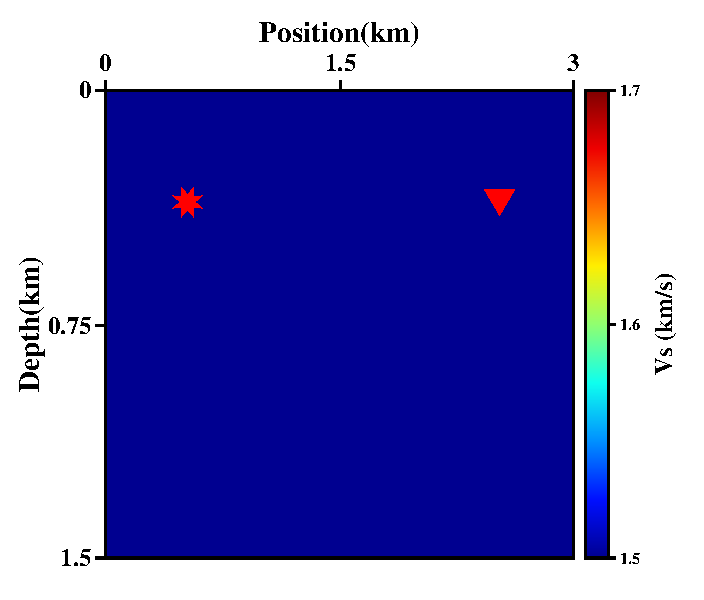
\includegraphics[width=0.50\textwidth]{Figure/chapter03/Kernel/1vs.pdf}}\\
   \subfloat[]{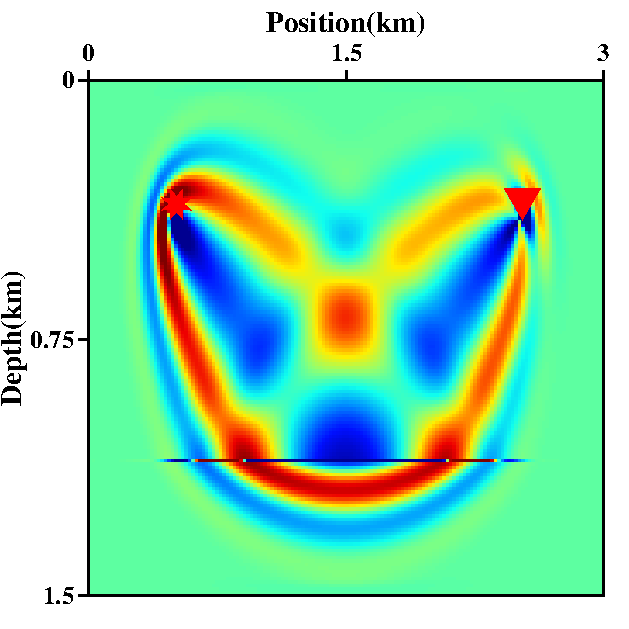
\includegraphics[width=0.50\textwidth]{Figure/chapter03/Kernel/Vponlyvp.pdf}}
   \subfloat[]{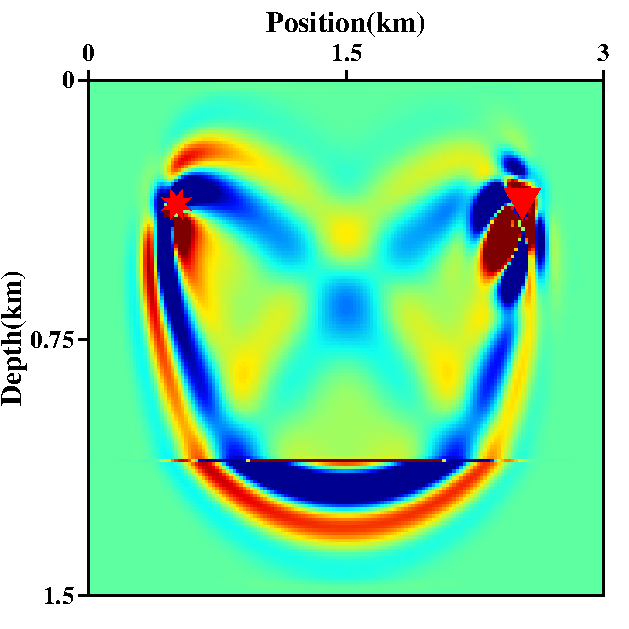
\includegraphics[width=0.50\textwidth]{Figure/chapter03/Kernel/Vsonlyvp.pdf}}\\
   \caption{单$V_p$界面的反射波路径。(a) $V_p$模型,(b) $V_s$模型,(c) $V_p$敏感核函数,(d) 
   $V_s$敏感核函数.}
   \label{fig:kernel1_vp}
\end{figure}

为了简化表达,将式\eqref{eq:GradientCijkl}重新写作:
\begin{equation}
    \nabla E(
    \mathbf{m}_0)=-\int(
    \mathbf{u}\cdot\delta \boldsymbol{\psi}
    +\delta
    \mathbf{u}\cdot{\boldsymbol{\psi}})
    \label{eq:kernelgradient} 
\end{equation} 
其中$\mathbf{u}$和$\boldsymbol{\psi}$为背景介质的正传与共轭波场,$\delta\mathbf{u}$和$\delta \boldsymbol{\psi}$为正传与共轭的散射场。
这里统一用$\cdot$表示波场分量的互相关。上式只示意性表达出反射波路径的计算方式,而不同参数化方式相应的具体计算公式需要参照链式法则获得。
上式中第一项表示震源到反射界面的波路径,第二项表示从反射界面到检波点的波路径。考虑到
波场解耦,上式的梯度也可以分解成P或S波数据组合的分量:
\begin{equation}
    K_m^{MN}     
    =-\int(\mathbf{u}^M\cdot\delta \boldsymbol{\psi}^N
    +\delta  \mathbf{u}^M\cdot\boldsymbol{\psi}^N),\\
    \label{eq:decompkernel} 
\end{equation}
其中$m\in\{V_p, V_s\}$,$M,N\in\{P,S\}$。

为了观察弹性波反射波路径(敏感核函数),先在单界面模型中计算反射波波路径。假定只有$V_p$的扰动界面(如图\ref{fig:kernel1_vp}a和b)。
%\begin{figure}
%   \centering
%   \subfloat[]{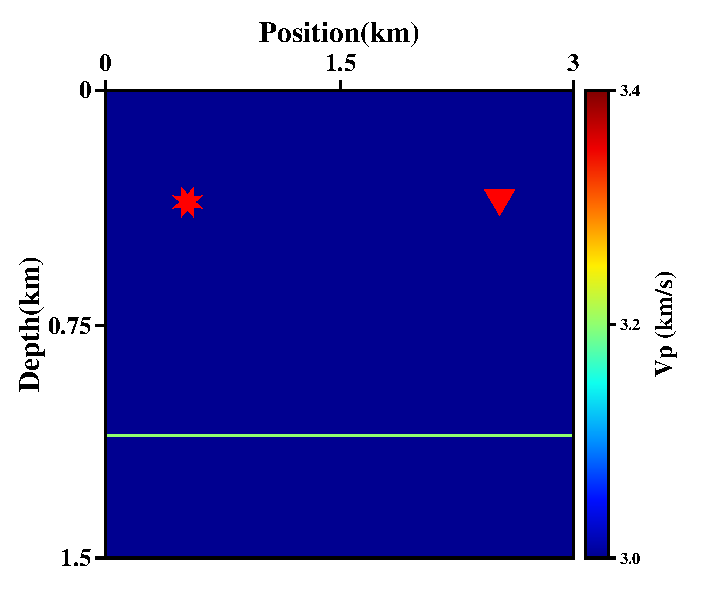
\includegraphics[width=0.38\textwidth]{Figure/chapter03/Kernel/1vp.pdf}}
%   \subfloat[]{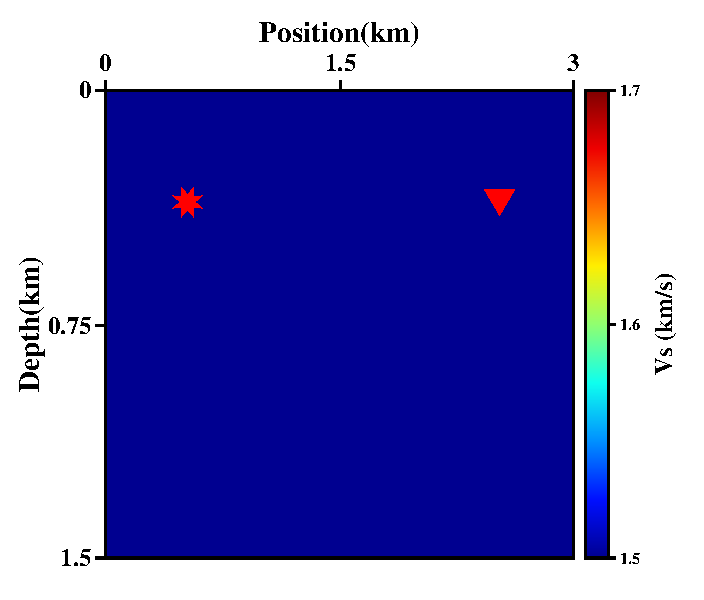
\includegraphics[width=0.38\textwidth]{Figure/chapter03/Kernel/1vs.pdf}}\\
%   \caption{单独$V_p$扰动界面。左侧为$V_p$,右侧为$V_s$.}
%   \label{fig:KernelModel1}
%\end{figure}
由于没有$V_s$扰动,因此没有模式转换能量而只有PP波反射,非常接近于声波情况。
采用该模型获得的反射波波路径如图\ref{fig:kernel1_vp}c和d。可以看到,$V_p$的反射波
路径分为震源端以及检波点端左右两支,与声波波路径非常接近。同时,$V_s$也会有相应的波路径能量,但是主要集中在边缘部分,第一菲涅尔带中央区域
能量较弱。原因可能是这部分波路径信息是与PP波反射能量对应的,对$V_s$背景信息并不敏感。
%如果换做$\lambda$和$\mu$的参数化方式,其产生的波路径如图\ref{Kernel1_lambda}所示
%\begin{figure}
%   \centering
%   \subfloat[]{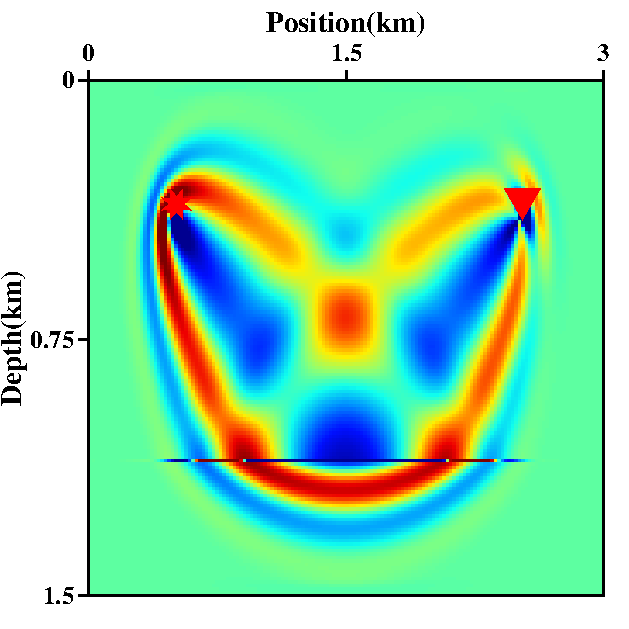
\includegraphics[width=0.30\textwidth]{Figure/chapter03/Kernel/lambdaonlyvp.pdf}}
%   \subfloat[]{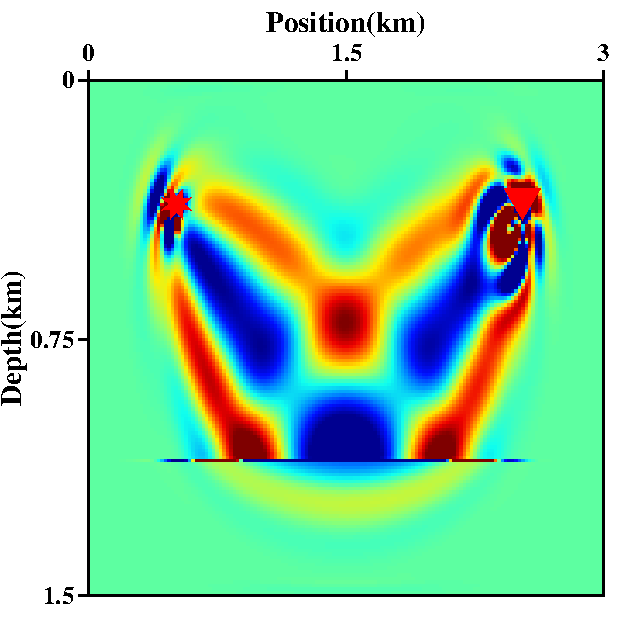
\includegraphics[width=0.30\textwidth]{Figure/chapter03/Kernel/muonlyvp.pdf}}\\
%   \caption{图\ref{fig:KernelModel1}模型$\lambda$参数化时的反射波路径。左侧为$\lambda$,右侧为$\mu$.}
%   \label{fig:kernel1_lambda}
%\end{figure}
\begin{figure}[!htb]
   \centering
   \subfloat[]{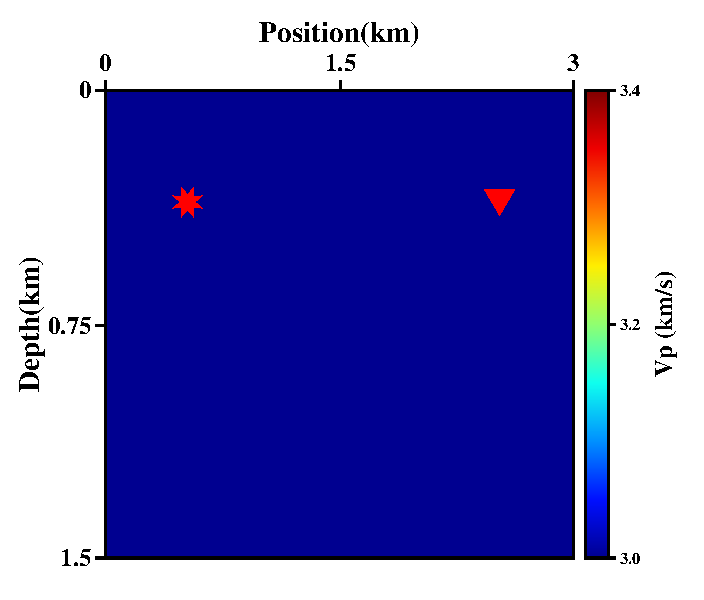
\includegraphics[width=0.50\textwidth]{Figure/chapter03/Kernel/2vp.pdf}}
   \subfloat[]{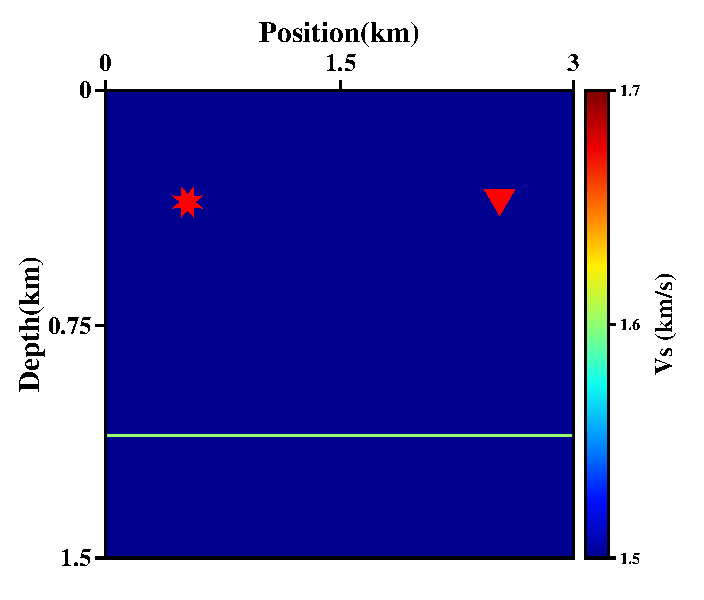
\includegraphics[width=0.50\textwidth]{Figure/chapter03/Kernel/2vs.pdf}}\\
   \subfloat[]{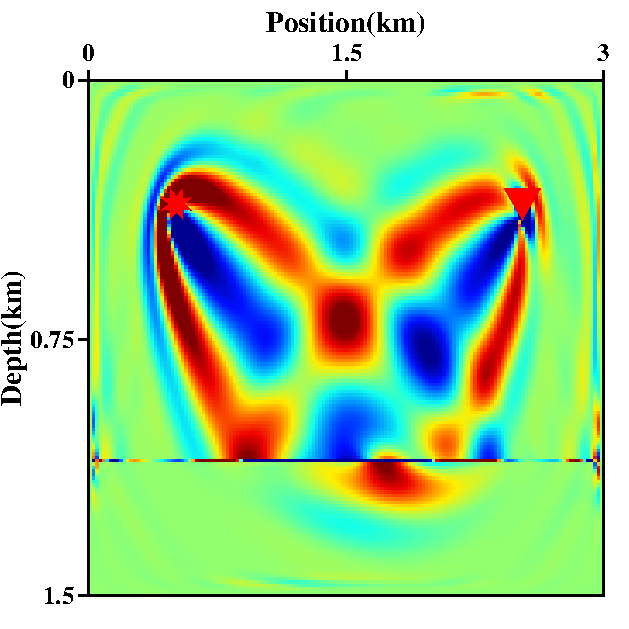
\includegraphics[width=0.50\textwidth]{Figure/chapter03/Kernel/Vponlyvs.pdf}}
   \subfloat[]{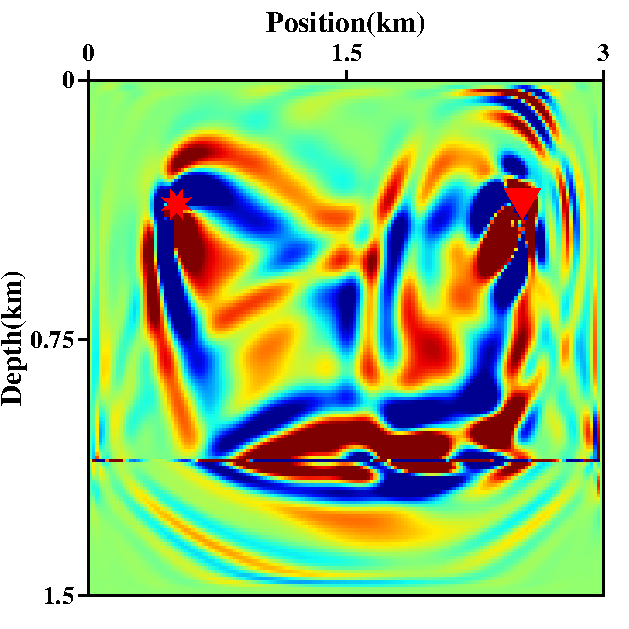
\includegraphics[width=0.50\textwidth]{Figure/chapter03/Kernel/Vsonlyvs.pdf}}\\
   \caption{单$V_s$界面的反射波路径。(a) $V_p$模型,(b) $V_s$模型,(c) $V_p$敏感核函数,(d) 
   $V_s$敏感核函数.}
%   \caption{单独$V_p$扰动界面。左侧为$V_p$,右侧为$V_s$.}
   \label{fig:kernel2}
\end{figure}

然后,考虑$V_s$模型存在界面的情况(图\ref{fig:kernel2}a和b)。此时波场就会变得十分复杂
,在正传及反传波场中会同时存在P波与S波,导致反射波路径变得更加复杂。
%\begin{figure}
%   \centering
%   \subfloat[]{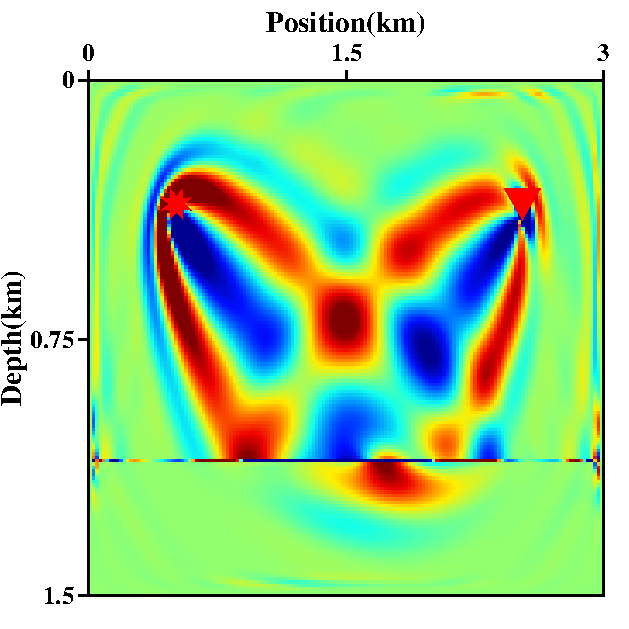
\includegraphics[width=0.30\textwidth]{Figure/chapter03/Kernel/Vponlyvs.pdf}}
%   \subfloat[]{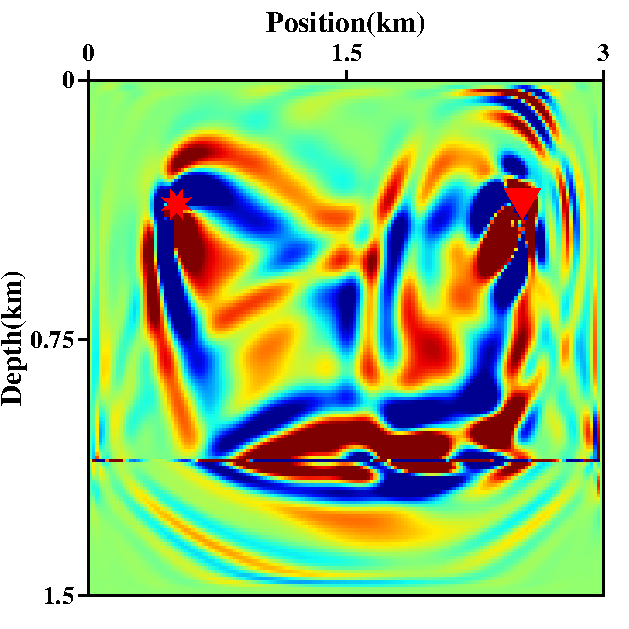
\includegraphics[width=0.30\textwidth]{Figure/chapter03/Kernel/Vsonlyvs.pdf}}\\
%   \caption{单独$V_p$扰动时的反射波路径。左侧为$V_p$,右侧为$V_s$.}
%   \label{fig:kernel2}
%\end{figure}
\begin{figure}[!htb]
   \centering
   \subfloat[]{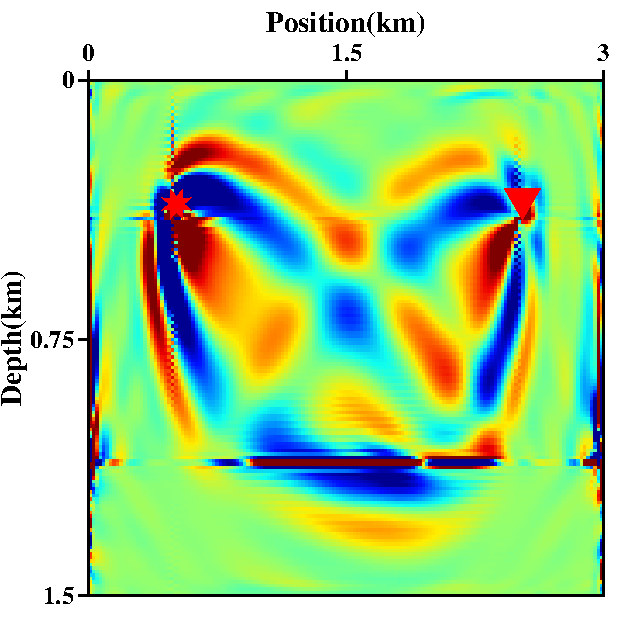
\includegraphics[width=0.50\textwidth]{Figure/chapter03/Kernel/VsonlyvsPP.pdf}}
   \subfloat[]{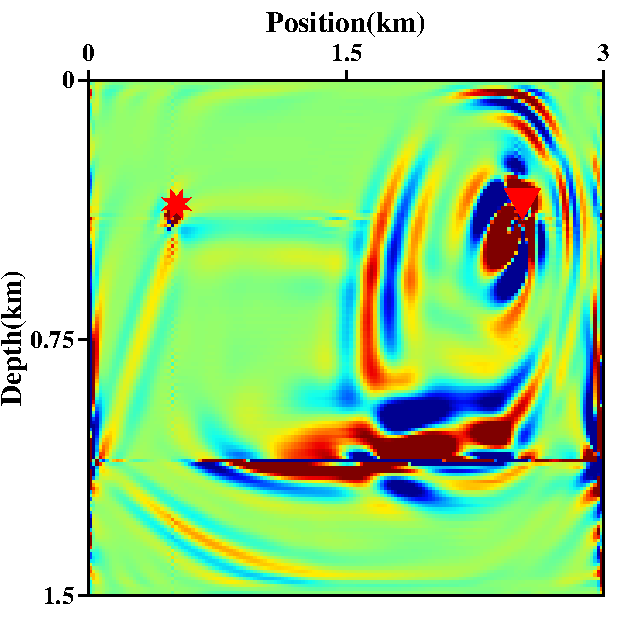
\includegraphics[width=0.50\textwidth]{Figure/chapter03/Kernel/VsonlyvsPS.pdf}}\\
   \subfloat[]{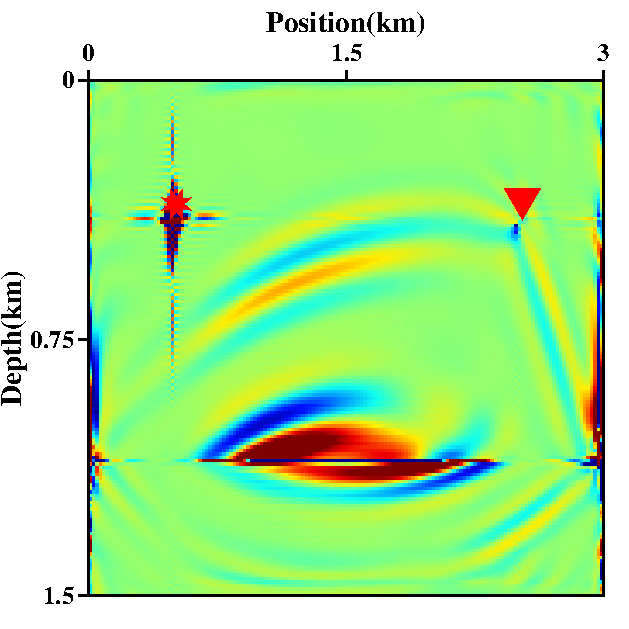
\includegraphics[width=0.50\textwidth]{Figure/chapter03/Kernel/VsonlyvsSP.pdf}}
   \subfloat[]{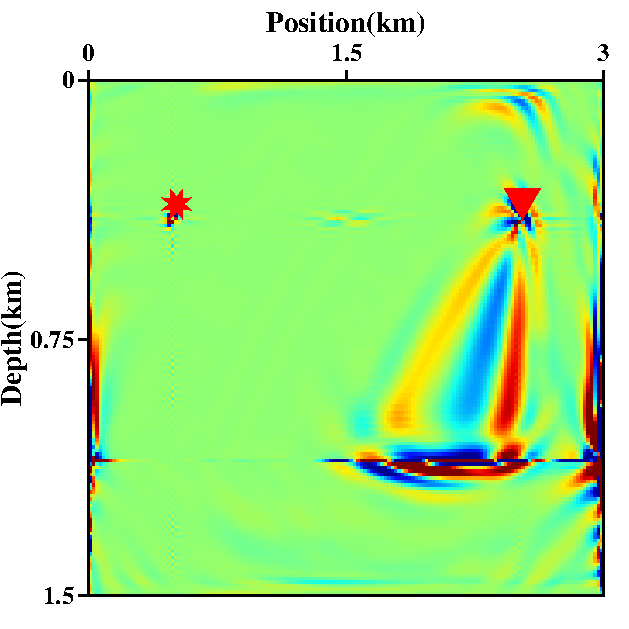
\includegraphics[width=0.50\textwidth]{Figure/chapter03/Kernel/VsonlyvsSS.pdf}}
   \caption{$K_{V_s}$敏感核函数的四个分量:(a) $K_{V_s}^{PP}$, (b) $K_{V_s}^{PS}$, (c) $K_{V_s}^{SP}$, (d) $K_{V_s}^{SS}$.}
   \label{fig:kernel2_vs_decomp}
\end{figure}
图\ref{fig:kernel2}中$V_p$敏感核函数与图\ref{fig:kernel1_vp}有所不同,这是因为当存在$V_s$反射界面时,反传的散射波场在界面处产生“非物理”的SP转换波,
这部分波场与背景场中的P波互相关就会产生一些假象。而在$V_s$的敏感核函数中,可以看到多种模式转换导致的多个波路径叠加,使得核函数十分复杂。
但是可以观察到其中的P波路径的能量总是占主导地位。
如果直接采用该核函数来计算目标函数关于$V_s$的梯度,一定会因为这些严重的cross-talk对反演带来更多的麻烦。

根据公式\eqref{eq:decompkernel},将原始的$V_s$核函数分解为四个部分。
如图\ref{fig:kernel2_vs_decomp}所示,$K_{V_s}^{PP}$与图\ref{fig:kernel2}c中
的$V_p$核函数十分类似,但是主要能量的符号相反(在第二章图\ref{fig:all}中有类似现象);$K_{V_s}^{PS}$与$K_{V_s}^{SP}$则包含非常多的高频信息,
它们主要是不同模式的正传与反传波场之间的偏移脉冲响应;$K_{V_s}^{SS}$则与其他三者有些不同,只包含了检波点端的单支反射路径,这是由于
采用了P波震源,在震源端的波场中不包含S波数据($K_{V_s}^{SS}$的震源端项会是0)。这样的话,$K_{V_s}^{SS}$就几乎不受到P波路径的影响。
如果利用这些后核函数分量的这些特征,
将会非常有助于背景$V_s$的反演。
\section{反射走时反演流程}
弹性介质中P波震源情况下,不同模式的转换波(主要是PP与PS波)同相轴之间会互相叠加、互相交叉。在用DIW提取走时残差的时候,这些交叉点的位置就会变成一些奇异点带来很大麻烦
。因此,如果直接用原始多分量数据的话,拾取到的$\tau(\mathbf{x_r},t;\mathbf{x_s})$就会不准确,这也是为什么式\eqref{eq:AdjointDeltaWE}中的梯度很难直接应用。
为了解决这个问题,本文将观测与模拟地震数据分解为P波与S波两部分。该模式分解只作用于地面地震数据\cite[]{Li2016a},可以快速地获得每一炮数据分解之后的矢量
P波或S波地震记录。这样,走时残差就可以被分成P波与S波两部分,使得弹性波WERTI变得可行。于是,设计出一个两阶段的反演流程,先P波阶段后S波阶段。
由于DIW提取走时的方式对数据的频率成分并不敏感,因此EWERTI中的多尺度策略主要体现在参数反演先后顺序上,并不需要过多考虑分频的策略。

$\quad$

$\quad$

$\quad$
\subsection{$V_p$反演}
在这个阶段主要采用PP反射波来建立P波速度的背景模型。首先,从ERTM中获得P波速度的扰动,即$\delta V_p$。
因为在速度不准的情况下大偏移距数据的偏移/反偏移结果会
造成模拟的反射波零偏移距走时误差,进而增加反演的非线性程度。
这里为了确保模拟数据与观测数据中零(小)偏移距反射走时相匹配,只采用小偏移距的数据
获取$\delta V_p$。
此外,由于在EWERTI中只考虑走时,可以只进行ERTM成像
而不是ELSRTM来估计反射率。
这也降低了反演中对反射系数估计的依赖程度。因此,目标函数变为最小化PP反射波的走时残差:
\begin{equation}
    E_{pp}=\frac{1}{2}\int\tau^2_{pp}(\mathbf{x_r},t;\mathbf{x_s})dtd\mathbf{x_r}d\mathbf{x_s}.
    \label{eq:ObjectivefunctionPP} 
\end{equation}
这样,采用分离的P波记录来计算方程\eqref{eq:AdjointWE}的右端项,并用$\delta V_p$替换方程\eqref{eq:DeltaWE}和\eqref{eq:AdjointDeltaWE}中的$\delta c_{ijkl}$,
就可以计算得到$V_p$的梯度($\frac{\partial E}{\partial V_p}$)。与EFWI一样,该梯度中的互相关项自动隐含了散度算子。因此,在
计算时只利用了PP反射波,所以不需要额外施加空间域的模式解耦。这个PP波走时反演本质上接近于声波反射走时反演,区别在于需要将地
面多分量地震记录进行数据域模式分离。注意,在分离后的数据中可能包含部分SP模式的转换波,它们对$V_p$的反演可能造成不利的影响,这需要今后更深入的研究。

\subsection{$V_s$反演}
接下来将对PS反射波采用类似的反演。相应地,目标函数变为:
\begin{equation}
    E_{ps}=\frac{1}{2}\int\tau^2_{ps}(\mathbf{x_r},t;\mathbf{x_s})dtd\mathbf{x_r}d\mathbf{x_s}.
    \label{eq:ObjectivefunctionPS} 
\end{equation}
值得一提的是,PS反射波的模拟(预测)方式与前一阶段略有不同。这里有两种方式来模拟PS反射波:

方式\uppercase\expandafter{\romannumeral1}: 采用反演好的$V_p$以及初始$V_s$模型来实现PS波偏移成像,然后使用该成像结果进行反偏移;

方式\uppercase\expandafter{\romannumeral2}: 由于$V_p$的背景速度在前一阶段已经被较好地恢复,此时PP波成像结果应该比较接近准确位置。考虑到大多数情况下,地
下介质中$V_p$与$V_s$的界面是比较一致的,因此也可以采用PP波成像结果作为界面来模拟PS反射波。

经过测试,发现第一种方式产生的近偏移距走时
对$V_p$模型的误差非常敏感,即使$V_p$模型在真值附近扰动也有可能获得方向错误的走时残差。
对于非对称的PS反射波的路径,假定地下存在如图\ref{fig:PS_refl}所示的单界面PS波反射。
由几何关系以及Snell定律,存在如下关系
%入射角$\theta_1$与反射角$\theta_2$之间以及深度、偏移距与该角度之间的关系为:
\begin{equation}
%\begin{split}
    \frac{sin\theta_1}{V_p}=\frac{sin\theta_2}{V_s},\qquad
    h(tan\theta_1+tan\theta_2)=X,
%\end{split}
    \label{eq:Snell_PS} 
\end{equation}
\begin{figure}
   \centering
   \subfloat{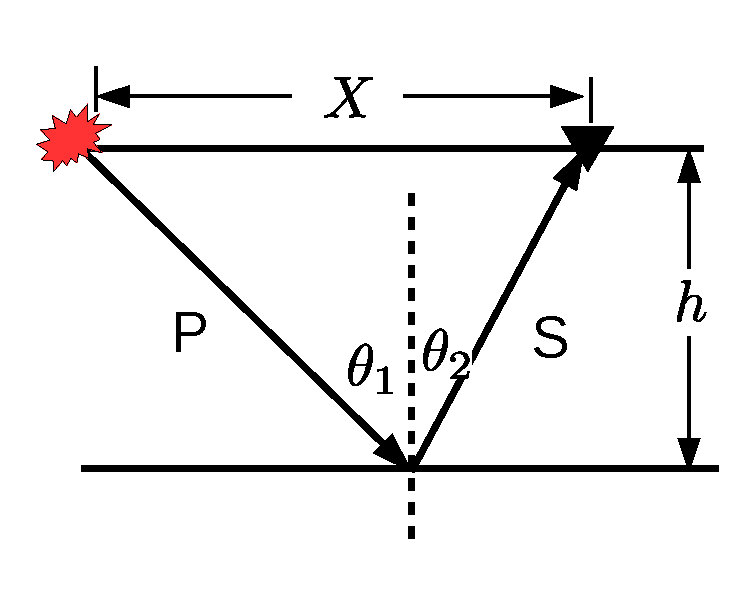
\includegraphics[width=0.40\textwidth]{Figure/chapter03/PS_problem/PS_refl.pdf}}
   \caption{单界面PS反射波示意图。}
   \label{fig:PS_refl}
\end{figure}
其中$\theta_1$和$\theta_2$分别为入射和反射角,$h$为界面深度,则PS波时距曲线关系为:
\begin{equation}
	t=\frac{h}{cos\theta_1V_p}+\frac{h}{cos\theta_2V_s}.
    \label{eq:TravelTime_PS} 
\end{equation}
方式\uppercase\expandafter{\romannumeral1}与方式\uppercase\expandafter{\romannumeral2}的差异在于速度不准时,确定界面深度的过程不同。
这里数值分析时使用零(小)偏移距的图偏移获得界面深度,然后带入到
式\eqref{eq:TravelTime_PS}中来近似获得错误速度下反偏移获得的反射数据的时距关系。

方式\uppercase\expandafter{\romannumeral1}
中,在图偏移时零偏移距走时保持不变,则偏移后的深度位置满足:
\begin{equation}
	\frac{h_{1}}{V_p}+\frac{h_{1}}{V^{'}_s}=\frac{h}{V_p}+\frac{h}{V_s},
    \label{eq:Mapmigration_PS} 
\end{equation}
其中$V^{'}_p$和$V^{'}_s$为错误的偏移速度。可以求得图偏移的深度:
\begin{equation}
	{h_{1}}=\frac{V^{'}_s(V_p+V_s)}{V_s(V^{'}_p+V^{'}_s)}h.
    \label{eq:ZerooffMig_PS} 
\end{equation}
而采用方式\uppercase\expandafter{\romannumeral2}时,在$V_p$存在误差时图偏移求得界面的深度为:
\begin{equation}
	{h_{2}}=\frac{V^{'}_p}{V_p}h.
    \label{eq:ZerooffMig_PP} 
\end{equation}
通常情况下
$V_p>V_s$因此$\frac{V_p+V_s}{V^{'}_p+V^{'}_s}$中$V^{'}_p$的小偏差也会带来很大的影响,
因此PS波零(小)偏移距成像界面的深度会同时受到$V_p$与$V_s$速度误差的影响。
下文将使用式\eqref{eq:Snell_PS}-\eqref{eq:ZerooffMig_PP}测试反偏移重建的反射数据的时距关系对$V^{'}_p$和$h$的敏感性。

这里将以下几个参数固定为$V_p=2500m/s$, $V_s=1500m/s$, $V^{'}_s=1300m/s$, 而$V^{'}_p$选取$2450,
2500, 2550m/s$三个扰动值。
从图\ref{fig:Sens_vp}可以看到,采用方式\uppercase\expandafter{\romannumeral1}时获取的反射数据对$V_p$的误差非常敏感,
在$\pm50m/s$范围内就会引起反偏移数据的走时残差改变方向
。相反,如果采用方式\uppercase\expandafter{\romannumeral2},其走时残差方向都是正确的。
\begin{figure}[h]
   \centering
   \subfloat[]{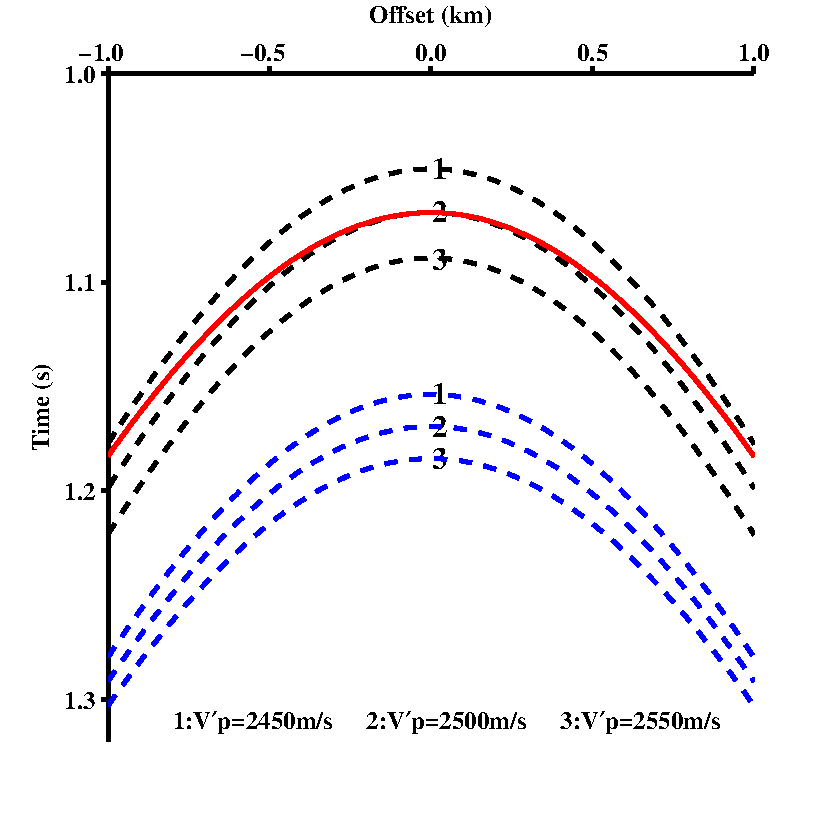
\includegraphics[width=0.5\textwidth]{Figure/chapter03/PS_problem/h1000.pdf}}
   \subfloat[]{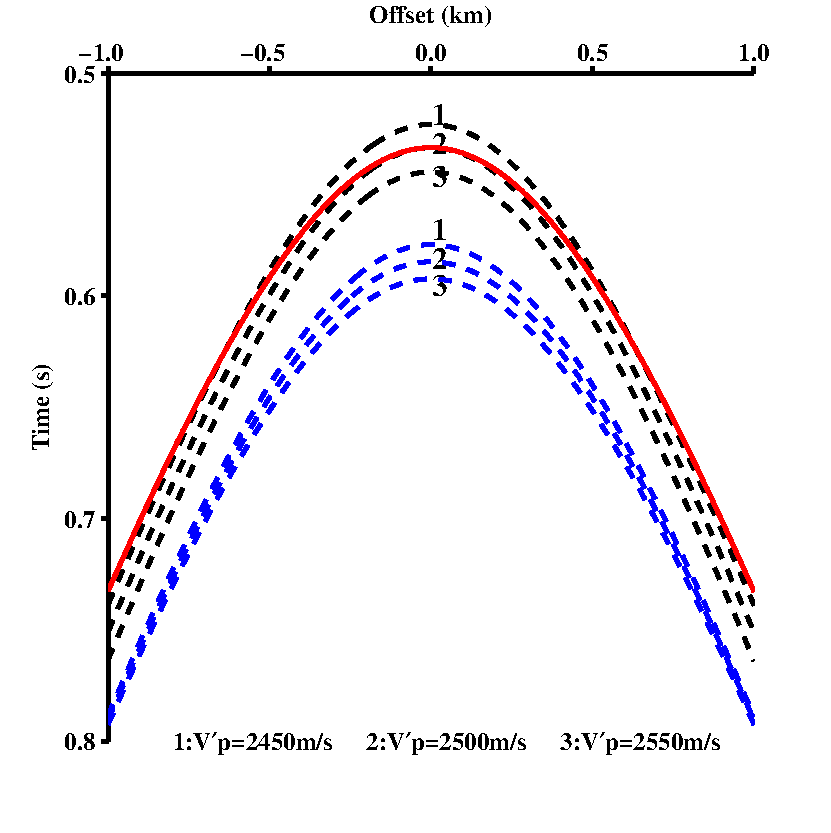
\includegraphics[width=0.5\textwidth]{Figure/chapter03/PS_problem/h500.pdf}}
   \caption{不同界面深度时方式\uppercase\expandafter{\romannumeral1}(黑色虚线)与
   方式\uppercase\expandafter{\romannumeral2}(蓝色虚线)反偏移获得PS波走时曲线
   与真实值(红色实线)之间的对比。数字1,2,3分别代表不同$V^{'}_p$速度的结果。(a) 界面深度$h=1000$; (b) 界面深度$h=500$.}
   \label{fig:Sens_vp}
\end{figure}

所以,本文采用较为准确的PP成像($\delta V_p$)结果
%而不
%是$\delta V_s$
来产生PS反射波。
但这样做也存在两个弊端:
第一、产生的PS反射无法保证振幅的准确性,幸运的是这并不会给DIW拾取走时残差带来大的
困扰;第二、来自深部的PS反射可能由于时差太大使得DIW拾取受到cycle-skipping困扰。
不过这个问题可以采用“层剥离”的方式,通过照明能量补偿的控制,先使用浅部的反射走时残差来更新浅层,
再使用深部的走时残差更新深部的速度。这样即使初始阶段深部的反射走时残差拾取错误也不影响浅部的速度更新。
在浅部更新较好后,深部的反射走时残差也能保证拾取得较为准确。
%先更新浅层$V_s$
%然后更新深层来避免。
%但方式\uppercase\expandafter{\romannumeral2}也存在问题,
%即在界面深度较深时,Born模拟的走时偏离真值较远,如果存在多个同相轴就会难以进行震相间的匹配,这样即使DIW也会受到
%cycle-skipping影响,但幸运的是界面深度较浅时,Born模拟走时与观测数据偏离并不远,这样的话可以层剥离的方式来从浅到深反演
%解决深层反射的震相匹配问题。

此外,正如前文核函数分析提到,PS反射中震源端波路径只与P波速度相关,
因此在计算$\frac{\partial E}{\partial V_s}$时可以丢掉方程\eqref{eq:GradientCijkl} 
右端项的第一部分。同时,波模式分解也会施加在梯度的计算过程中来确保只有S波能量参与计算,即:
\begin{equation}
    \frac{\partial E_{ps}}{\partial V_s}=-2\rho V_s
    \int (\frac{\partial \delta u^S_{i}}{\partial
    x_j}\frac{\partial \psi^S_{k}}{\partial x_l})
    (\delta_{ik}\delta_{jl}+
    \delta_{il}\delta_{jk}).
    \label{eq:GradientVel_S}
\end{equation}
该模式解耦的梯度与Wang et al.
(2015)\cite{wang:2015}提出的EFWI预条件方式类似,可以在$V_s$的反演中降低参数耦合的影响

\section{局部倾角导引正则化}
数据域的WERTI与成像域射线走时层析有一些相似特性。通常,射线走时层析由于射线路径覆盖不均匀、反射界面深度与速度之间存在耦合等问题会导致反演的多解性,
所以射线层析通常不收敛或者很难收敛到正确的速度模型。
常规各向同性平滑算子的正则化约束可以一定程度上降低上述多解性的困扰,但是也很难保证反演收敛到具有地质含义的物理模型。
在偏移后,成像结果可以提供地下界面大致的倾角信息,由此设计正则化算子来沿地层倾角对反演进行约束可以
有效地应对多解性的问题,从而加快收敛速度、改善反演结果。由于采用波动方程作为波场传播引擎,WERTI采用波路径信息来反投影走时残差,因而所面临的多解性挑战要
小于射线走时层析。不过,对于一些照明不足或者
反射路径覆盖不均匀的区域同样也会产生多解性问题。因此,WERTI中采用局部倾角导引的正则化同样可以加速
收敛,并获得具有地质意义的反演结果。

Hale (2009)\cite{Hale2009Structure}采用结构张量来估计地层倾角。对于2D的图像,结构张量是$2\times2$的矩阵:
\begin{equation}
        \mathbf{S}=
        \begin{pmatrix}
                < s^2_1 > \quad <s_1s_2 >\\
                < s_1s_2 > \quad < s^2_2 >\\
        \end{pmatrix},
        \label{eq:StructureTensor}
\end{equation}
其中$s_1$和$s_2$表示图像垂直和水平方向的方向导数,$<\dot>$表示2D的Gaussian平滑函数。上式对应的特征值问题可以表示为:
\begin{equation}
	\mathbf{S}=\lambda_u\mathbf{u}\mathbf{u}^T+\lambda_v\mathbf{v}\mathbf{v}^T
        \label{eq:EigenValueVector}
\end{equation}
其中$\lambda_u$和$\lambda_v$分别为特征向量$\mathbf{u}$和$\mathbf{v}$对应的特征值。定义$\lambda_u\ge\lambda_v\ge0$,这样的话$\mathbf{u}$指示梯度最大的
方向,即与线性结构垂直的方向,而$\mathbf{u}$则指示与线性结构平行的方向。Hale(2009)\cite{Hale2009Structure}指出,可以设置$\lambda_u(\mathbf{x})=0$
和$\lambda_v(\mathbf{x})=1$,保证图像中每一处平滑都会沿倾角方向。于是,沿倾角平滑的滤波器可以通过以下方程求解:
\begin{equation}
	(\mathbf{B}^T\mathbf{B}+\mathbf{A}^T\mathbf{S}^{\prime}\mathbf{A})\mathbf{h}=\mathbf{B}^T\mathbf{B}\mathbf{f}
        \label{eq:SparseMatrixSystem}
\end{equation}
其中$\mathbf{S}^{\prime}$为新构造的结构张量,$\mathbf{B}$和$\mathbf{A}$分别为求和算子以及差分算子对应的矩阵,$\mathbf{f}$为输入图像,$\mathbf{h}$
为输出的平滑后图像。该方程可以通过共轭梯度法快速求解,这样就可以采用以上方式对EWERTI的梯度进行正则化约束,大大缩小反演的零空间,保证收敛到更合理的结果。

\section{数值实验}
\subsection{目标函数性态分析}
事实上,除了DIW提取走时之外,空间或者时间方向上的互相关也经常用来作为提取走时拟合差的方法\cite{vanLeeuwen:2010,chi2015,Wang2015},其目标函数为:
\begin{equation}
\left\{
	\begin{aligned}
		&\Delta t(h)=\mathop{\arg\min}_{\Delta t}\int d^{o}(t+\Delta t,h)d^{c}(t,h)dt,\\
	&E_t=\frac{1}{2}\sum\parallel \Delta t(h)\parallel ^2
	\end{aligned}
	\right.
    \label{eq:Obj_TimeCorr} 
\end{equation}
或
\begin{equation}
\left\{
	\begin{aligned}
		&\Delta h(t)=\mathop{\arg\min}_{\Delta h}\int d^{o}(t,h+\Delta h)d^{c}(t,h)dt,\\
	&E_h=\frac{1}{2}\sum\parallel \Delta h(t)\parallel ^2
	\end{aligned}
	\right.
    \label{eq:Obj_SpatialCorr} 
\end{equation}
互相关提取的时差反映每一道或每一时刻数据的全局平均效果。
如果数据中反射同相轴比较多时,互相关反映出来的时差并不能体现局部某一个同相轴的运动学趋势。这就导致在模型复杂的时候,很难应对多震相的问题。
对比式\eqref{eq:Objectivefunction}可以发现,DIW衡量的则是局部的走时差异,具备更高的分辨能力。

下面将对比
在不同模型复杂程度下以上三种目标函数的性态差异。
由于PS波走时匹配需要采用层剥离逐步逼近,该过程较为复杂,因此这里只对PP波走时目标函数性态进行分析。采用常速背景+反射
系数的方式通过Born正演获得反射波数据,然后扰动背景速度,通过偏移/反偏移的方式模拟反射数据并由此计算目标函数值。
\begin{figure}
   \centering
   \subfloat[]{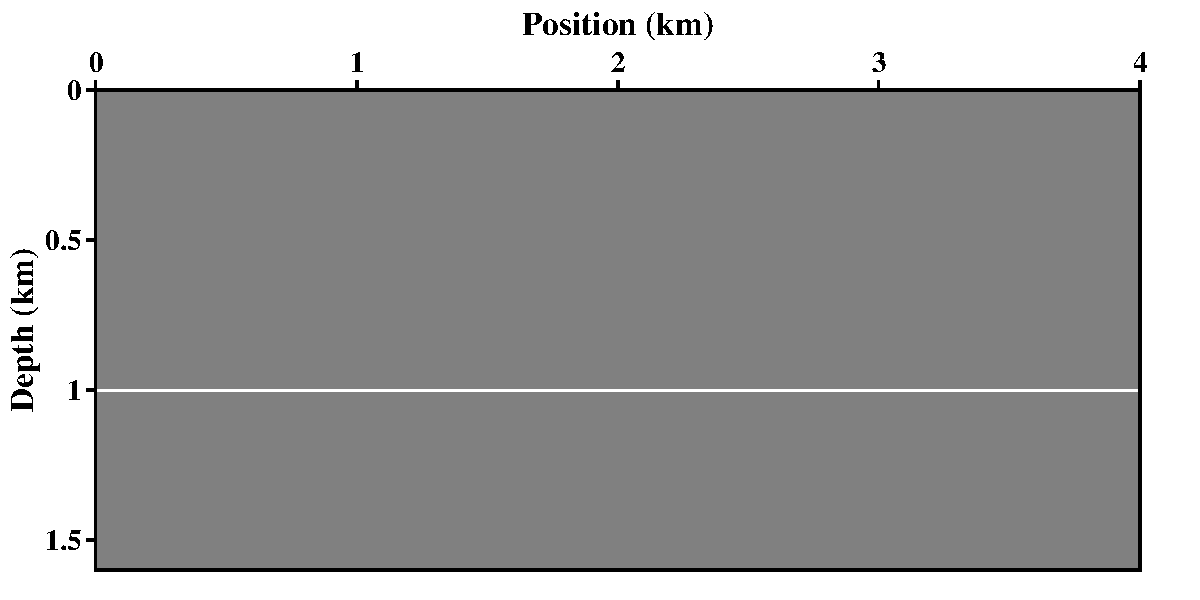
\includegraphics[width=0.5\textwidth]{Figure/chapter03/DIW_L2/1layer.pdf}}
   \subfloat[]{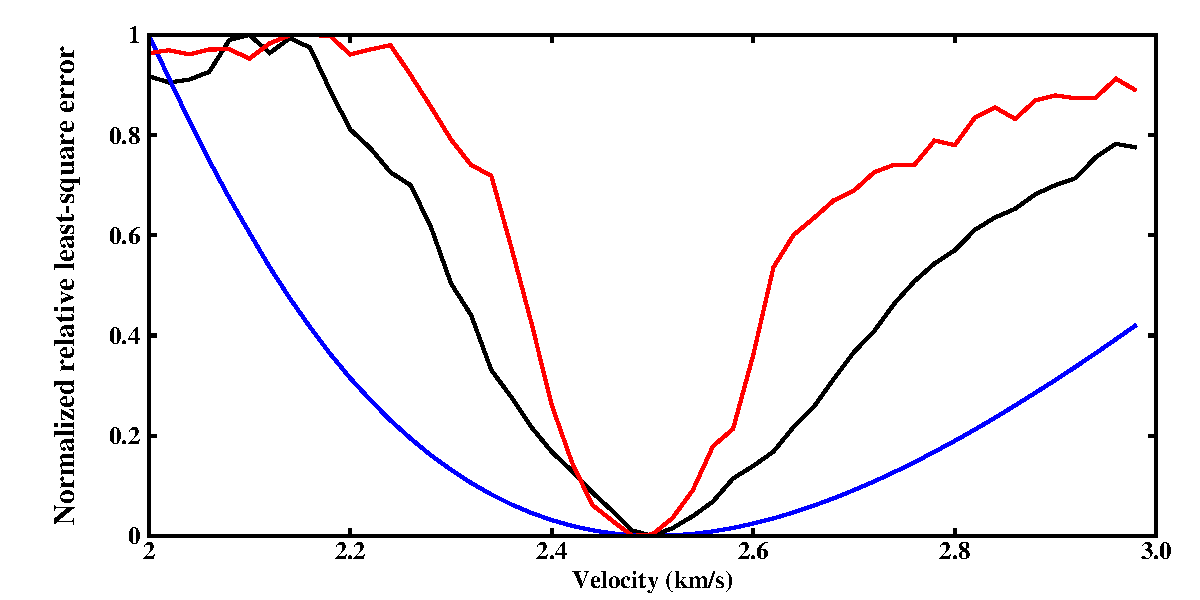
\includegraphics[width=0.5\textwidth]{Figure/chapter03/DIW_L2/1layerL2.pdf}}\\
   \subfloat[]{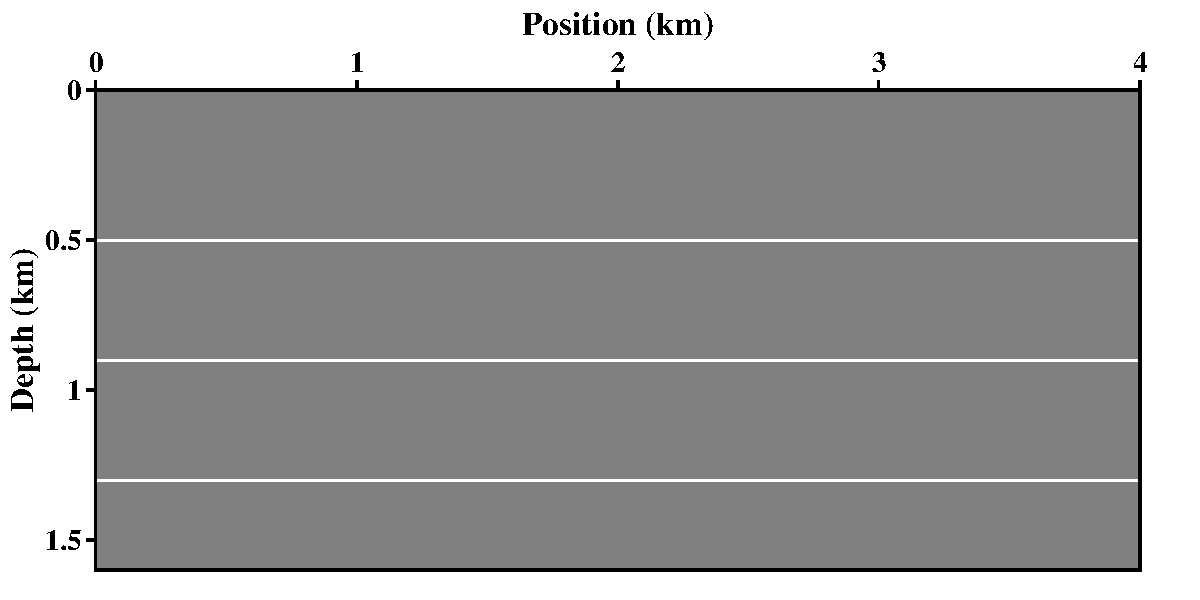
\includegraphics[width=0.5\textwidth]{Figure/chapter03/DIW_L2/3layer.pdf}}
   \subfloat[]{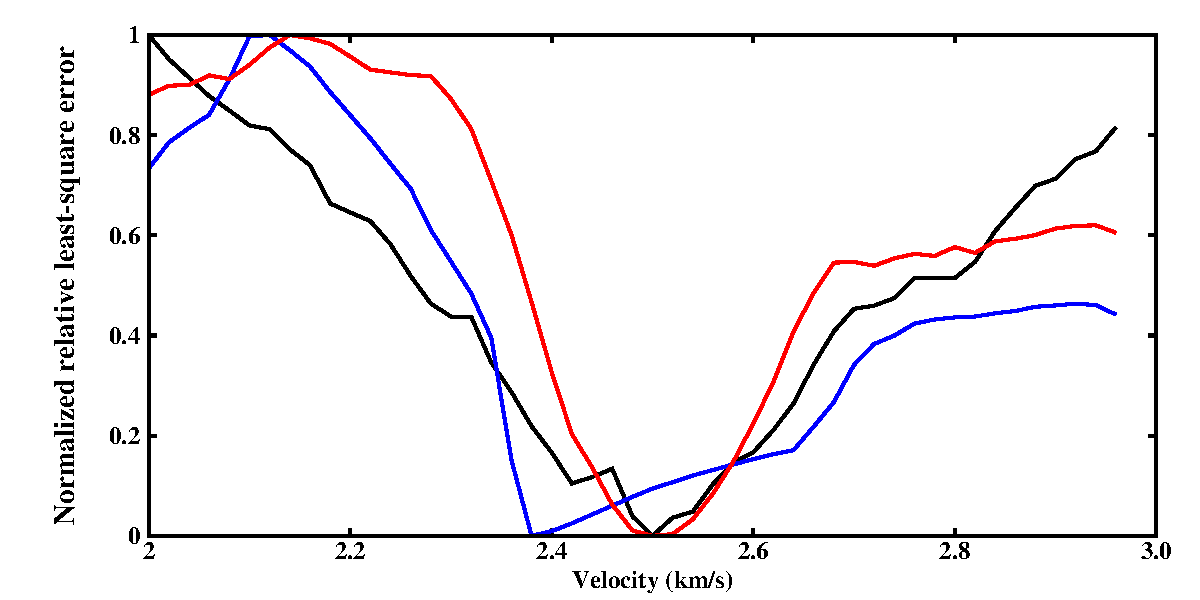
\includegraphics[width=0.5\textwidth]{Figure/chapter03/DIW_L2/3layerL2.pdf}}\\
   \subfloat[]{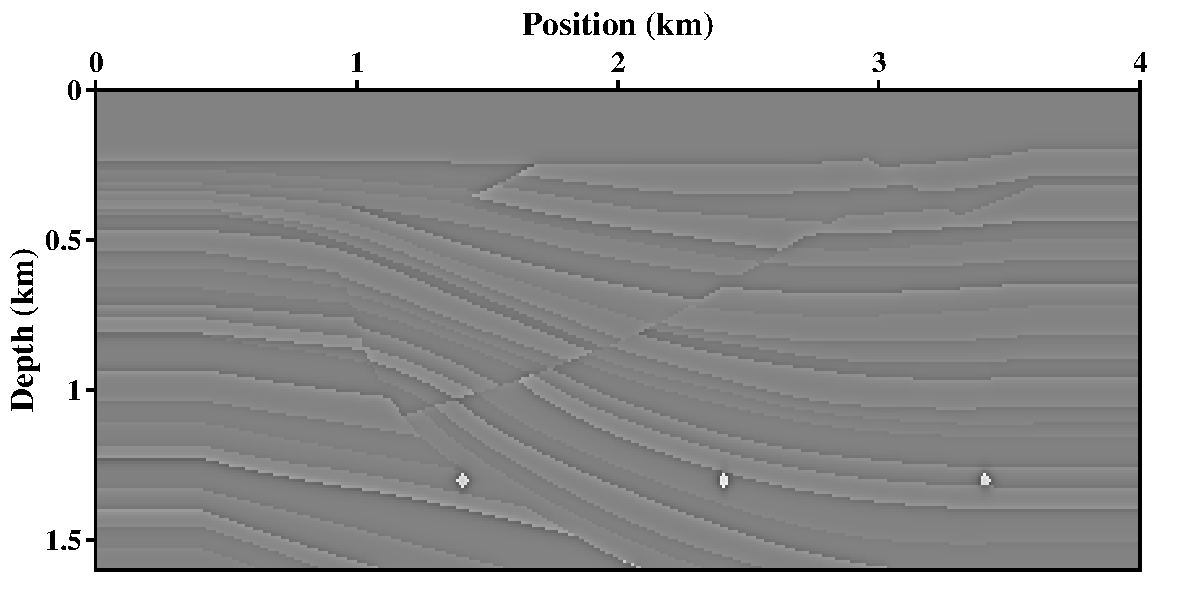
\includegraphics[width=0.5\textwidth]{Figure/chapter03/DIW_L2/Sigsbee.pdf}}
   \subfloat[]{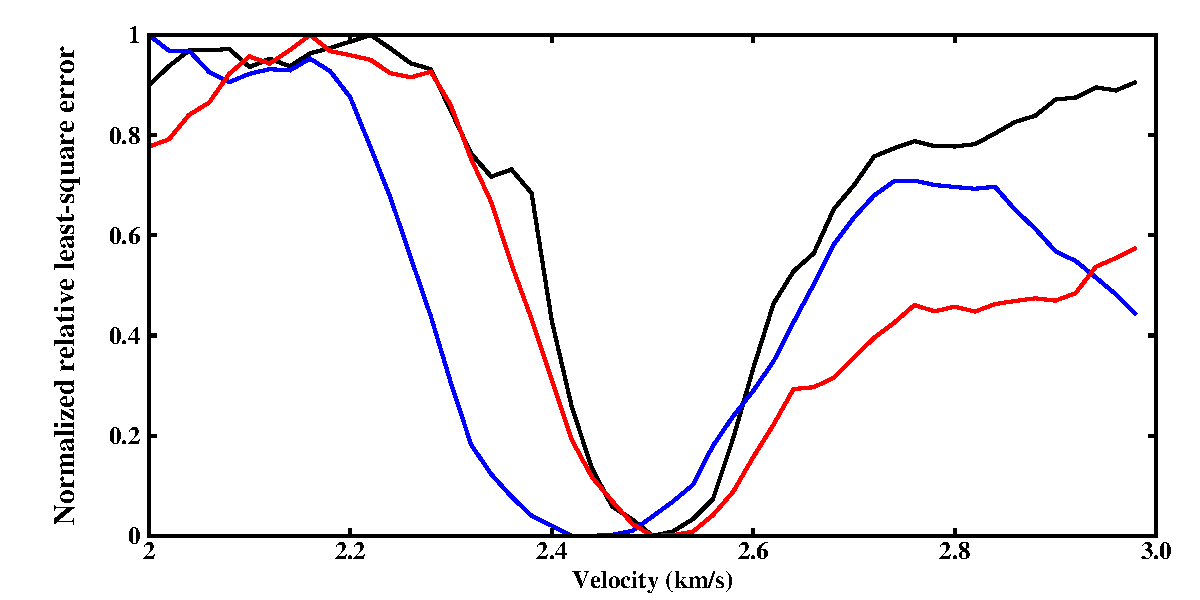
\includegraphics[width=0.5\textwidth]{Figure/chapter03/DIW_L2/complexL2.pdf}}
   \caption{不同模型及对应的PP波走时目标函数变化曲线。红色,蓝色和黑色分别对应DIW,时间互相关与空间互相关走时提取方式。}
   \label{fig:DIW_L2}
\end{figure}
三种不同模型对应的目标函数性态如图\ref{fig:DIW_L2}。
可见,在单界面时,反射同相轴单一,可区分度很高。由于DIW为局部数据匹配,其计算也会受到cycle-skipping影响。
此时,时间和空间互相关的目标函数表现要优于DIW。在三层模型中,由于反射同相轴变多,空间和时间互相关的目标函数准确性下降。空间互相关方式在
真值附近出现了局部极值,而时间互相关由于更难反映出时差随深度的变化,
其极值点出现在了错误的数值附近。但是DIW方式的稳定性并未随之明显降低,只是在速度偏大时对速度变化
不敏感,这也是由于受到cycle-skipping影响。

最后使用更为复杂的Sigsbee2A模型(局部)来试验(图\ref{fig:DIW_L2}e、f)。
可以看到时间互相关目标函数的极值点仍然偏离准确值较远,
空间互相关目标函数也变得对初始模型更加敏感,而基于DIW的目标函数的性态在复杂构造下仍然变化不大,尤其在速度偏高时的表现要优于相关类的目标函数,
说明它的收敛性相对更加稳健。
以上分析结果表明DIW方式构建走时残差目标函数在复杂区域更可靠,但是也会一定程度上受到cycle-skipping的影响。

\begin{figure}[!htb]
   \centering
   \subfloat[]{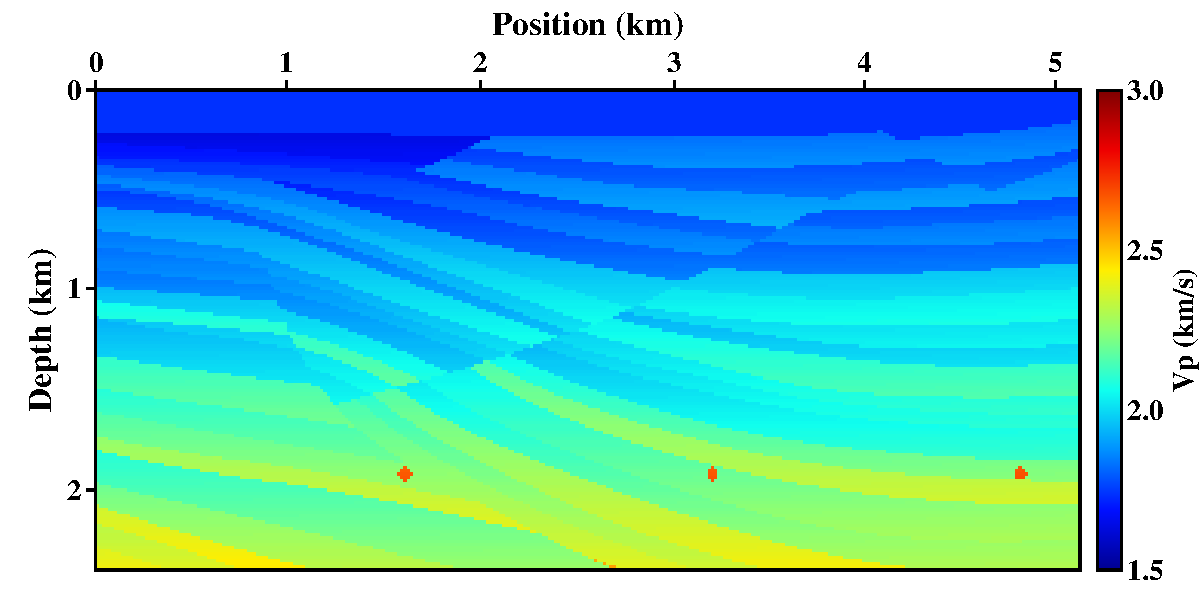
\includegraphics[width=0.5\textwidth]{Figure/chapter03/sigbee2/Fig/cuttruevp.pdf}}
   \subfloat[]{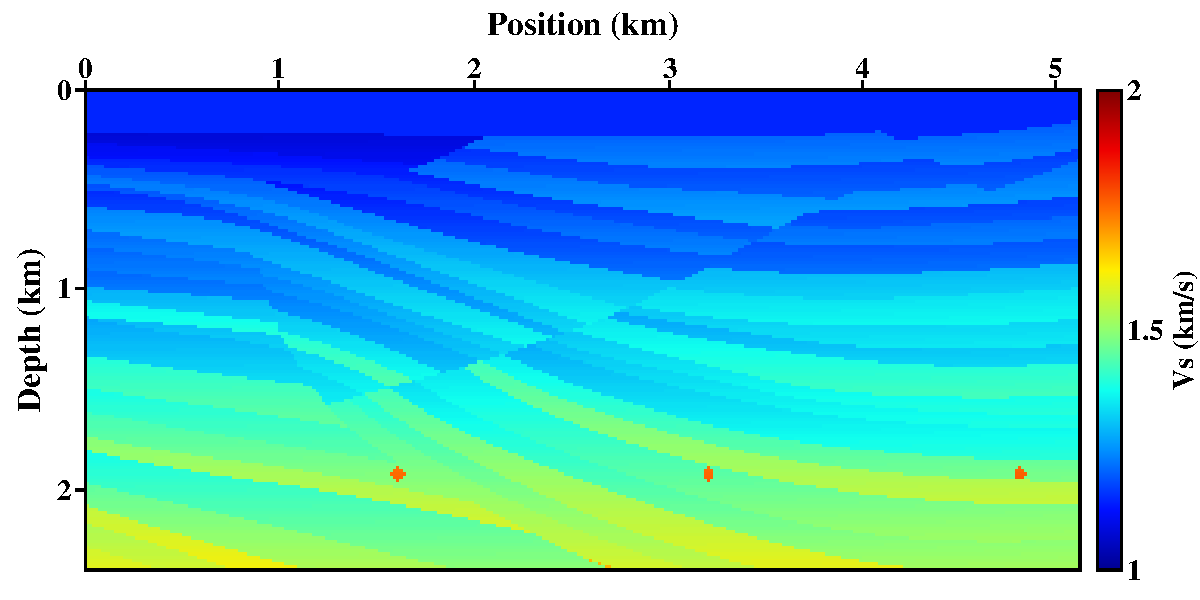
\includegraphics[width=0.5\textwidth]{Figure/chapter03/sigbee2/Fig/cuttruevs.pdf}}\\
   \subfloat[]{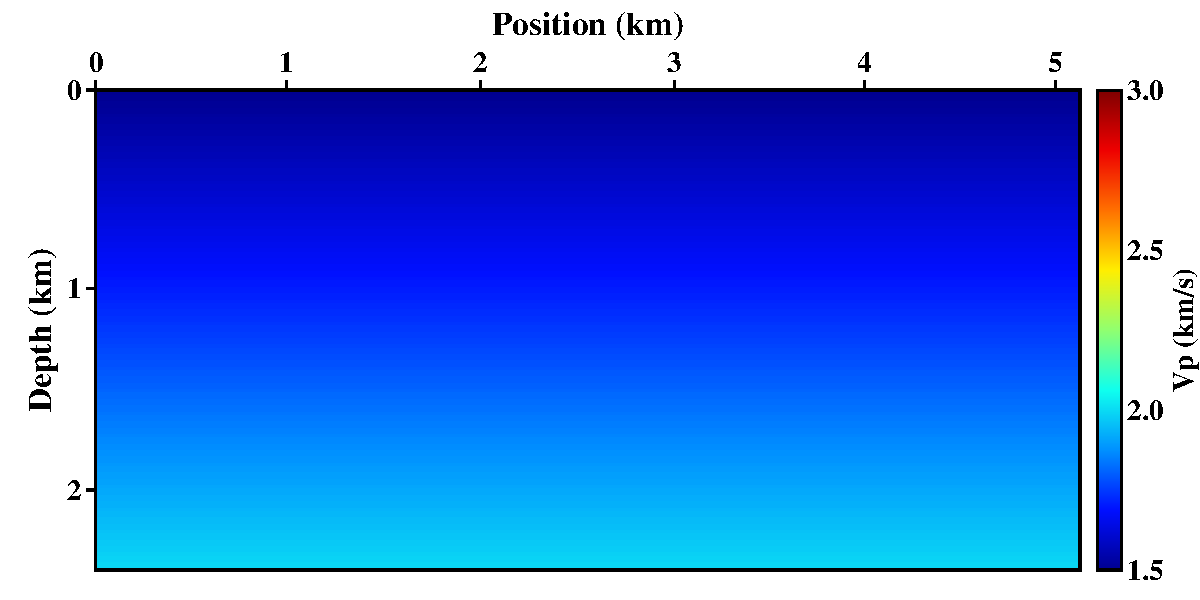
\includegraphics[width=0.5\textwidth]{Figure/chapter03/sigbee2/Fig/cutinitvp.pdf}}
   \subfloat[]{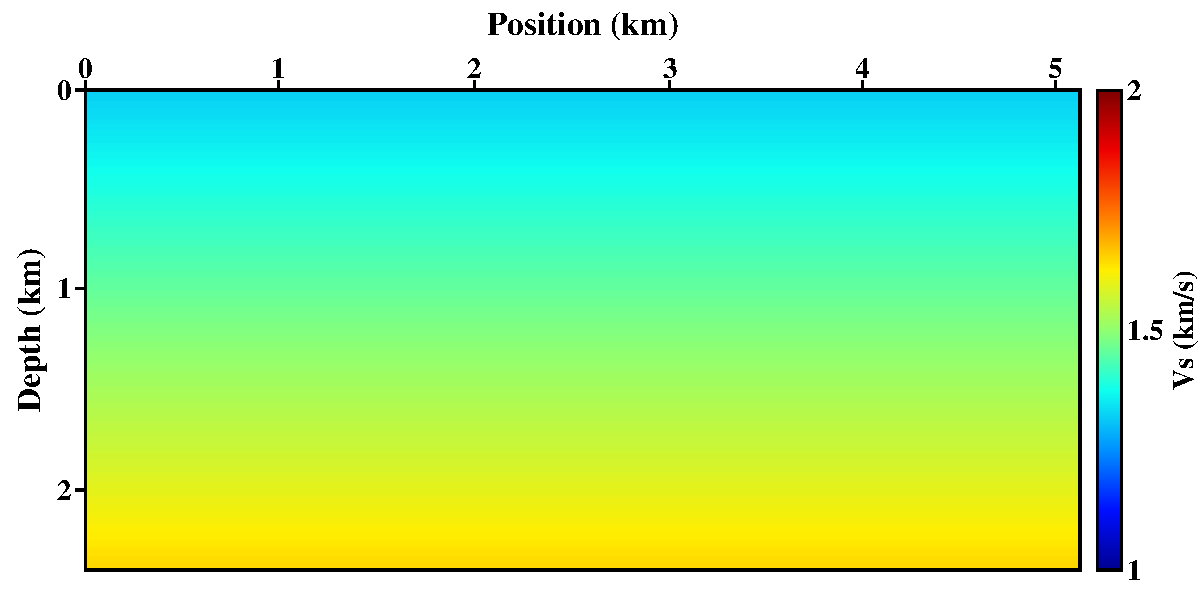
\includegraphics[width=0.5\textwidth]{Figure/chapter03/sigbee2/Fig/cutinitvs.pdf}}
   \caption{Sigbee2A真实$V_p$(a)和$V_s$(b)模型与初始$V_p$ (c)和$V_s$(d)模型。}
   \label{fig:TrueAndInitial}
\end{figure}
\subsection{Sigsbee2A模型}
为了验证EWERTI算法的有效性,本节采用Sigsbee2A模型的一部分来进行实验(如图\ref{fig:TrueAndInitial}a和\ref{fig:TrueAndInitial}b),
$V_s$模型通过固定的泊松比由$V_p$模型变换产生。
图\ref{fig:TrueAndInitial}c和\ref{fig:TrueAndInitial}d展示了$V_p$和$V_s$的初始模型,
速度值随深度线性增加。可以看到,初始模型中$V_p$比真实值偏低而$V_s$则偏高,
但这两者都偏离真实值较远。
观测数据模拟采用交错网格有限差分求解方程\eqref{eq:WE_3}。
水平和深度方向上空间采样均为16m,时间采样为1.2毫秒,接收时间为3.6s。
36个炮点均匀的分布在地表,检波点也布放在地表,最大偏移距为4km,震源子波主频为15Hz。实验中采用纯P波震源。
%初始模型的成像结果

\begin{figure}[!htb]
   \centering
   \subfloat[]{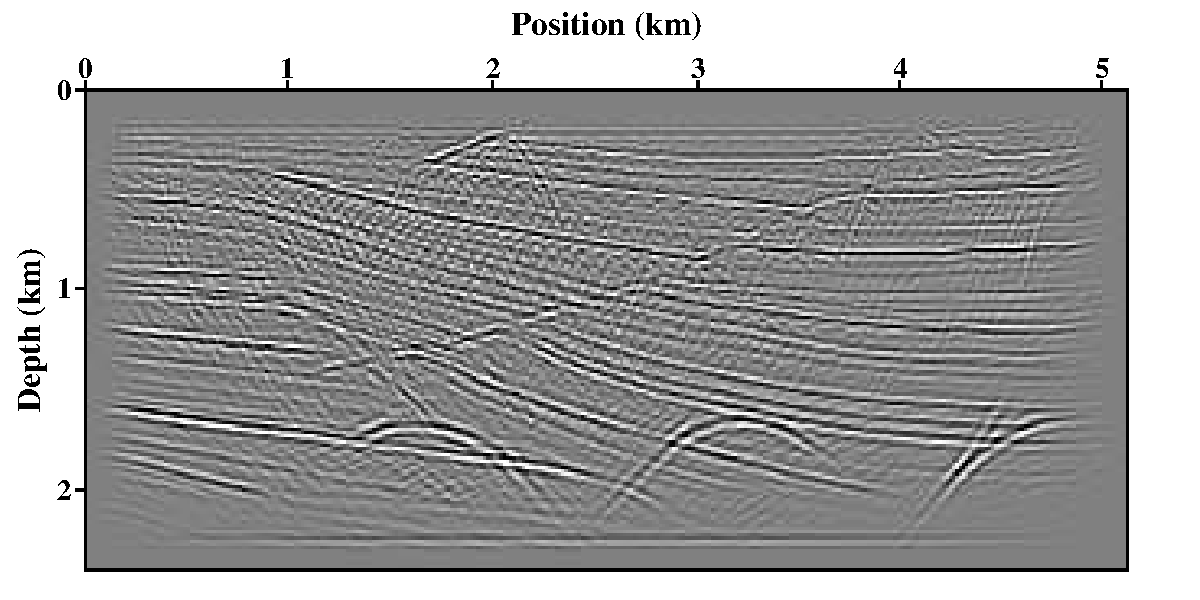
\includegraphics[width=0.5\textwidth]{Figure/chapter03/sigbee2/Fig/cutimage_initvp.pdf}}
   \subfloat[]{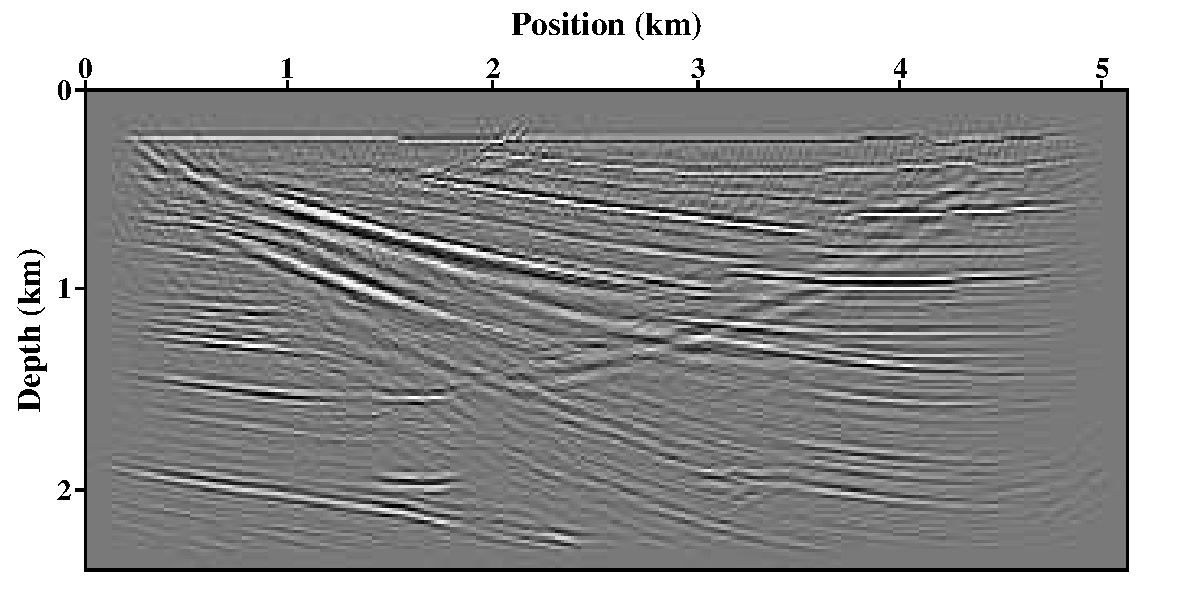
\includegraphics[width=0.5\textwidth]{Figure/chapter03/sigbee2/Fig/cutimage_initvs.pdf}}\\
   \subfloat[]{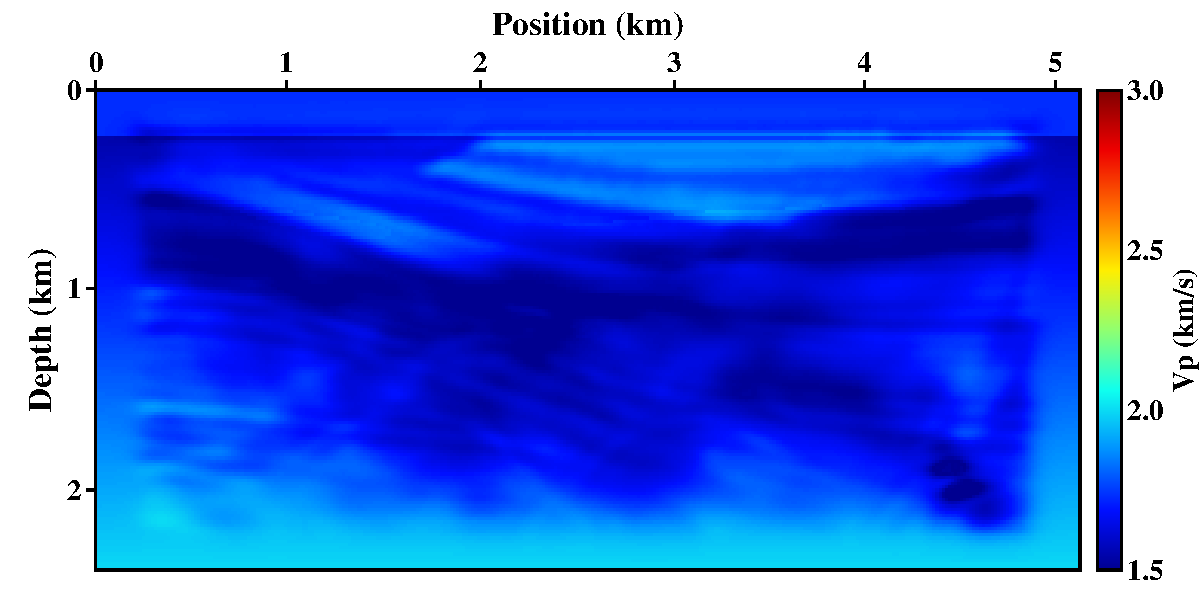
\includegraphics[width=0.5\textwidth]{Figure/chapter03/sigbee2/badinitvp.pdf}}
   \subfloat[]{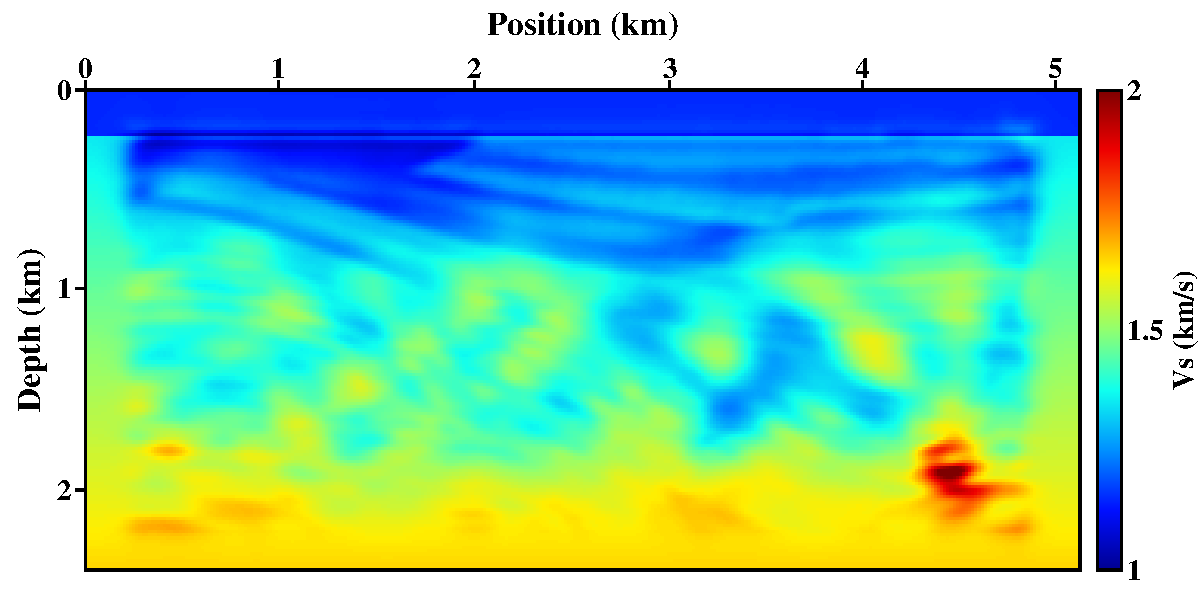
\includegraphics[width=0.5\textwidth]{Figure/chapter03/sigbee2/badinitvs.pdf}}\\
   \caption{初始模型下的ERTM与EFWI结果:(a)和(b)分别为小偏移距PP与PS波ERTM结果,(c)和(d)分别为EFWI估计的$V_p$与$V_s$}
   \label{fig:Results_init}
\end{figure}
\begin{figure}[!htb]
   \centering
   \subfloat[]{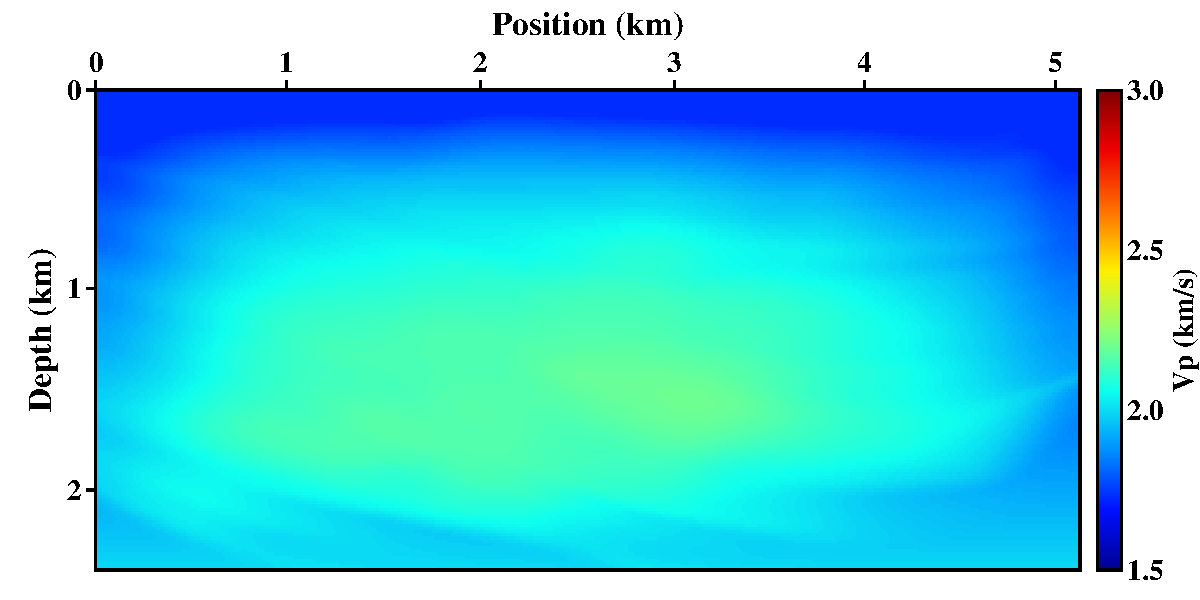
\includegraphics[width=0.5\textwidth]{Figure/chapter03/sigbee2/Fig/newinit3vp.pdf}}
   \subfloat[]{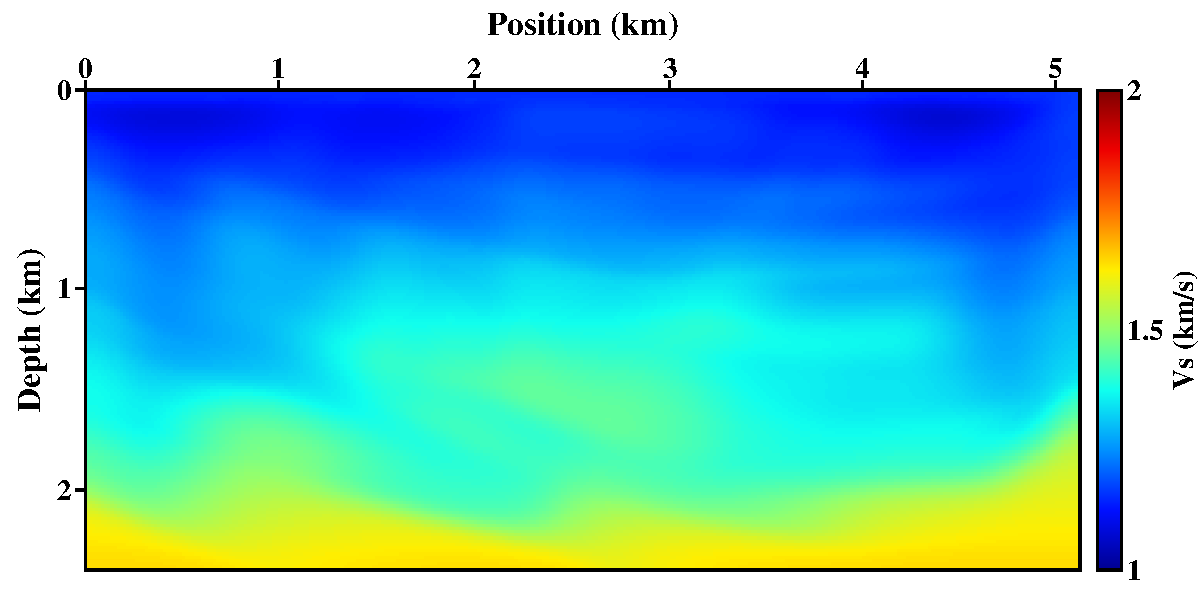
\includegraphics[width=0.5\textwidth]{Figure/chapter03/sigbee2/Fig/newinit3vs.pdf}}\\
   \caption{EWERTI反演模型:(a) $V_p$, (b) $V_s$.}
   \label{fig:InvertedModel_WERTI}
\end{figure}
%由于我们采用的初始模型随深度线性增大,其偏离真实值较远。
图\ref{fig:Results_init}为基于初始模型的ERTM与EFWI结果。可以看到小偏移距ERTM成像结果中界面位置全部错位,绕射波没有收敛。
%PP与PS波成像结果都无法估计准确反射界面位置。
如果采用该初始模型进行EFWI,
在浅部区域由于透射波的贡献还能够恢复出部分速度结构,但是随着深度的增加,速度中低波数成分不正确导致cycle-skipping问题严重,EFWI很快
陷入局部极值。

从上述不太好的初始模型出发,按照前文所设计的工作流程进行EWERTI,其反演结果如
图\ref{fig:InvertedModel_WERTI}。
在经过每个阶段40次迭代之后,EWERTI较好地恢复了模型中深部的中低波数成分,加之由于倾角导引正则化的贡献,
反演模型在宏观上与真实模型更吻合。但是模型两侧反射数据覆盖较少的区域以及最底部无反射波穿过的区域,
%由于缺乏反射波路径信息
EWERTI也无法对背景速度进行更新。
\begin{figure}[!htb]
   \centering
   \subfloat[]{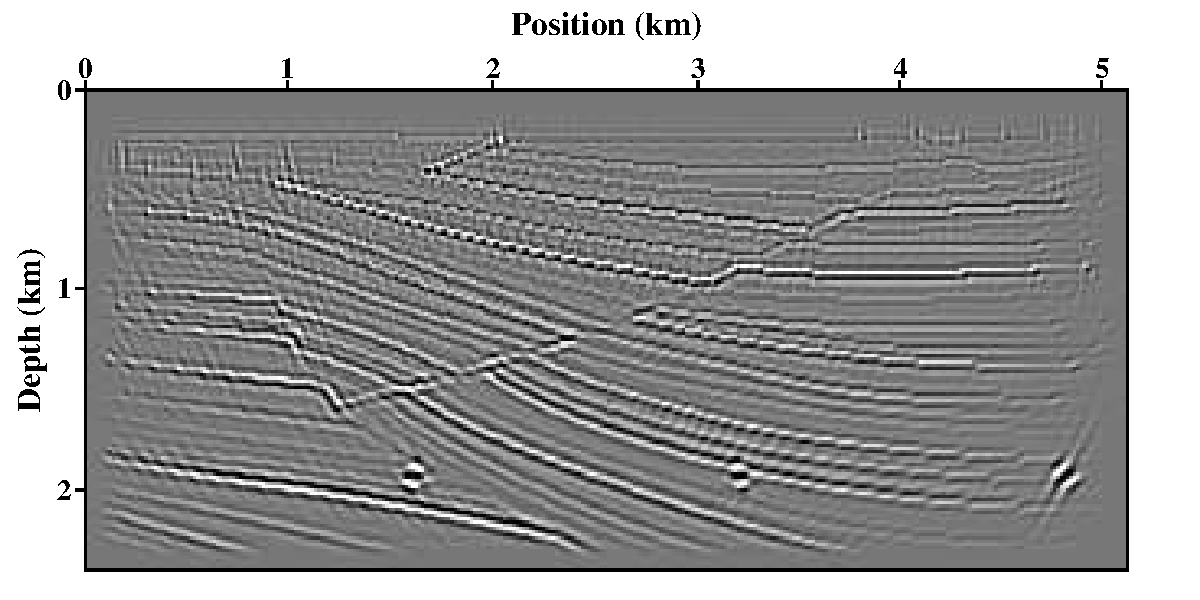
\includegraphics[width=0.5\textwidth]{Figure/chapter03/sigbee2/Fig/cutimage_truevp.pdf}}
   \subfloat[]{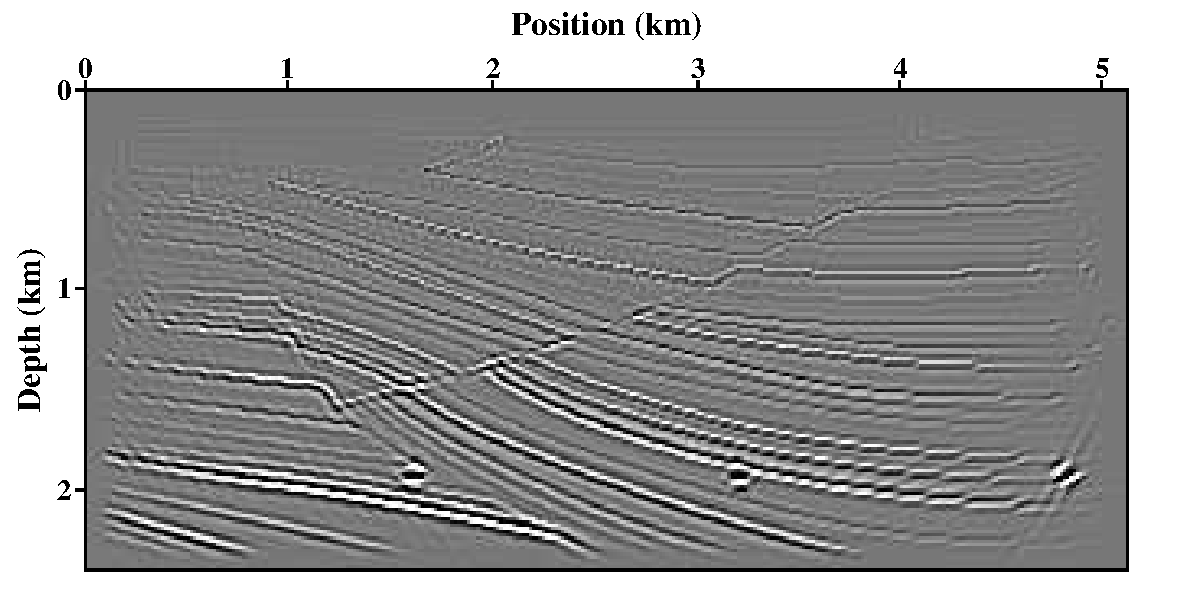
\includegraphics[width=0.5\textwidth]{Figure/chapter03/sigbee2/Fig/cutimage_truevs.pdf}}\\
   \subfloat[]{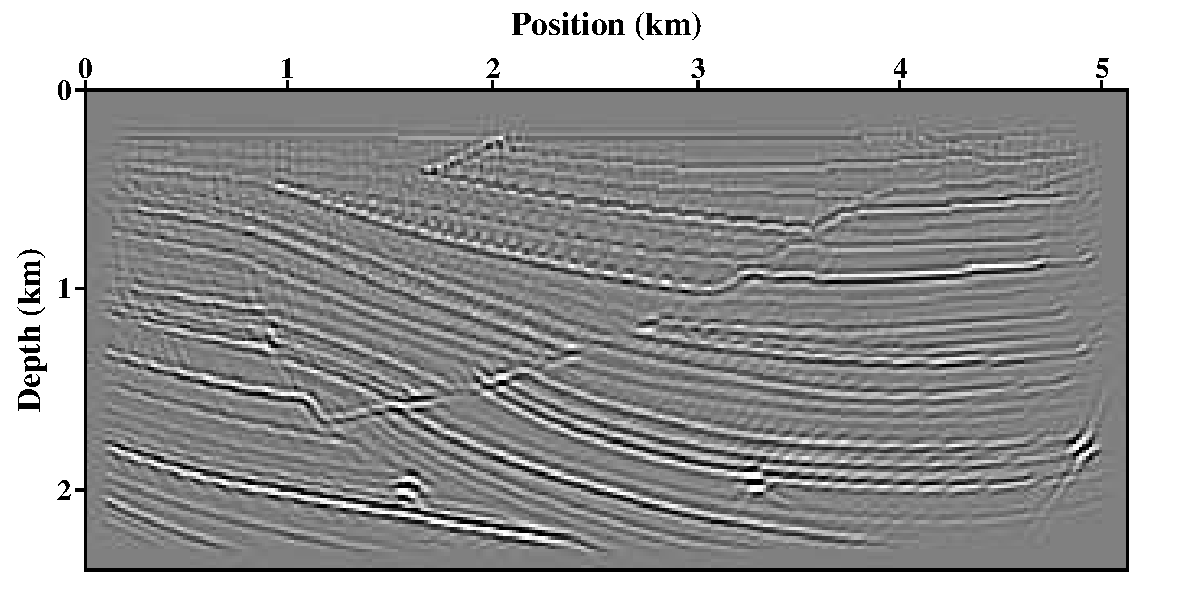
\includegraphics[width=0.5\textwidth]{Figure/chapter03/sigbee2/Fig/cutimage_wertivp.pdf}}
   \subfloat[]{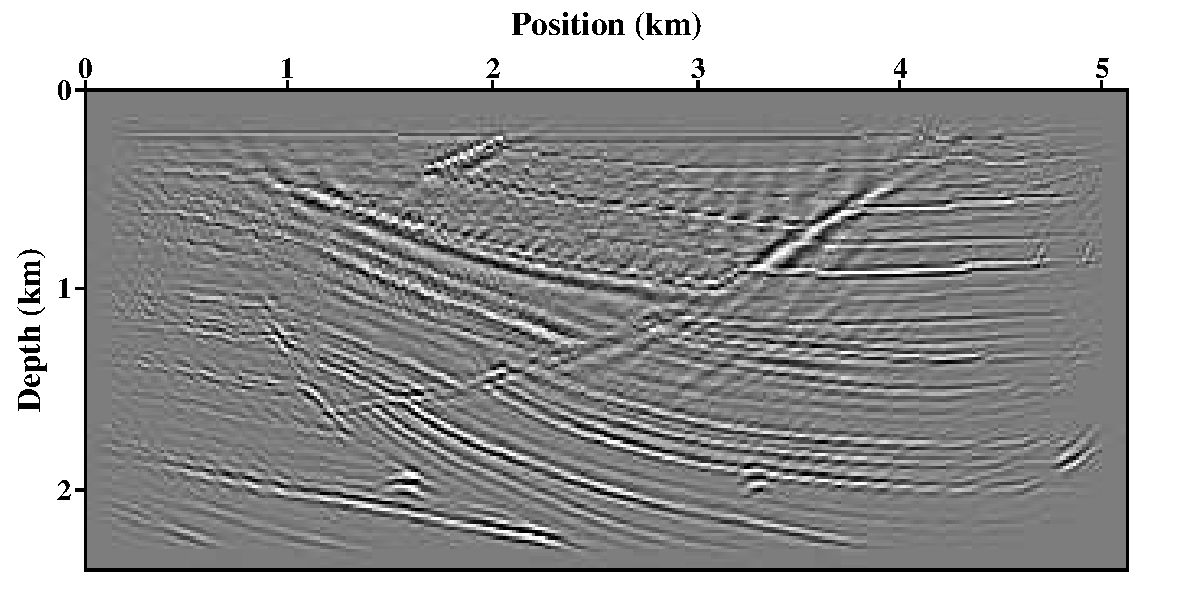
\includegraphics[width=0.5\textwidth]{Figure/chapter03/sigbee2/Fig/cutimage_wertivs.pdf}}
   \caption{真实模型与EWERTI反演模型的ERTM结果对比:(a)和(b)分别为真实模型PP与PS波ERTM结果;(c)和(d)分别为EWERTI模型PP与PS波ERTM结果。}
   \label{fig:ERTM_comparison}
\end{figure}
\begin{figure}[!htb]
   \centering
   \subfloat[]{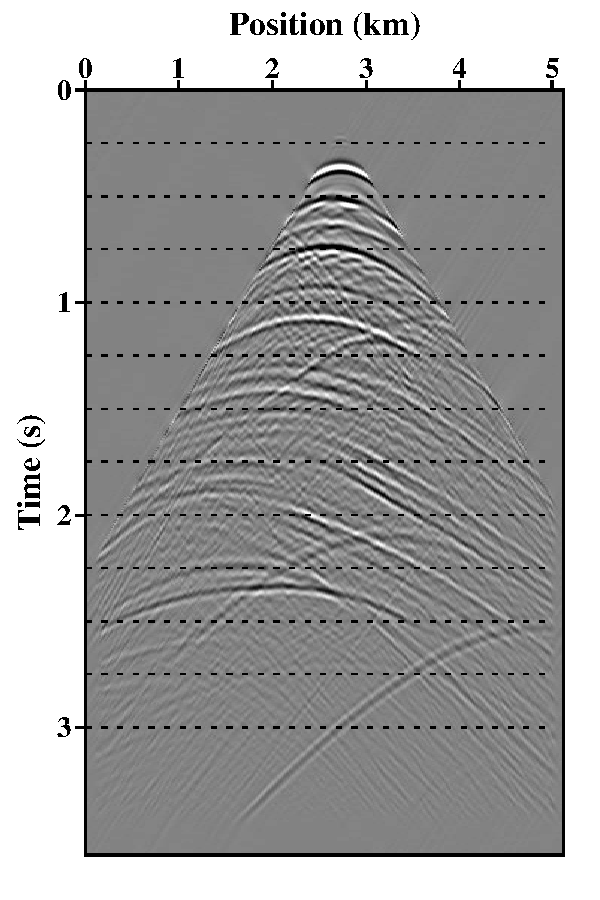
\includegraphics[width=0.33\textwidth]{Figure/chapter03/sigbee2/Fig/DataPP_true.pdf}}
   \subfloat[]{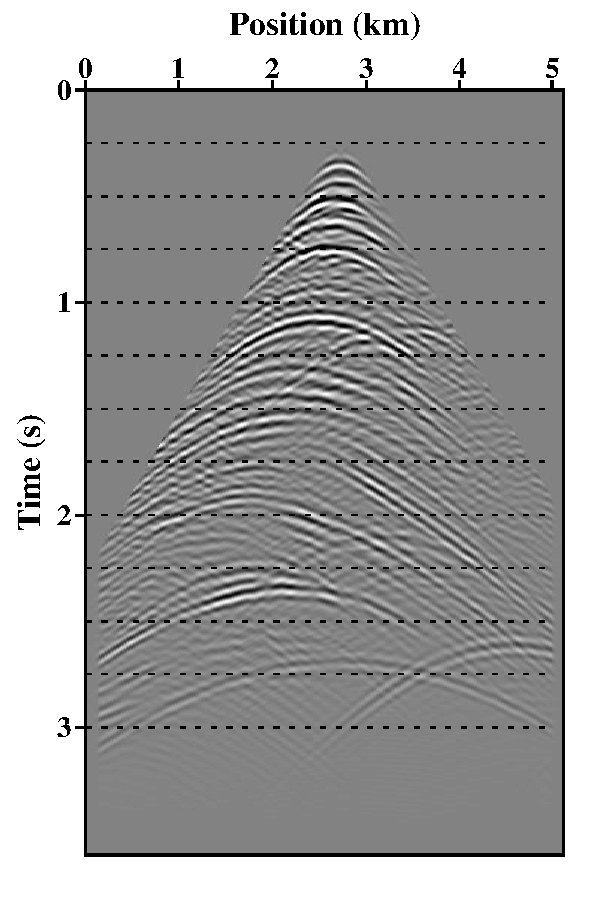
\includegraphics[width=0.33\textwidth]{Figure/chapter03/sigbee2/Fig/DataPP_init.pdf}}
   \subfloat[]{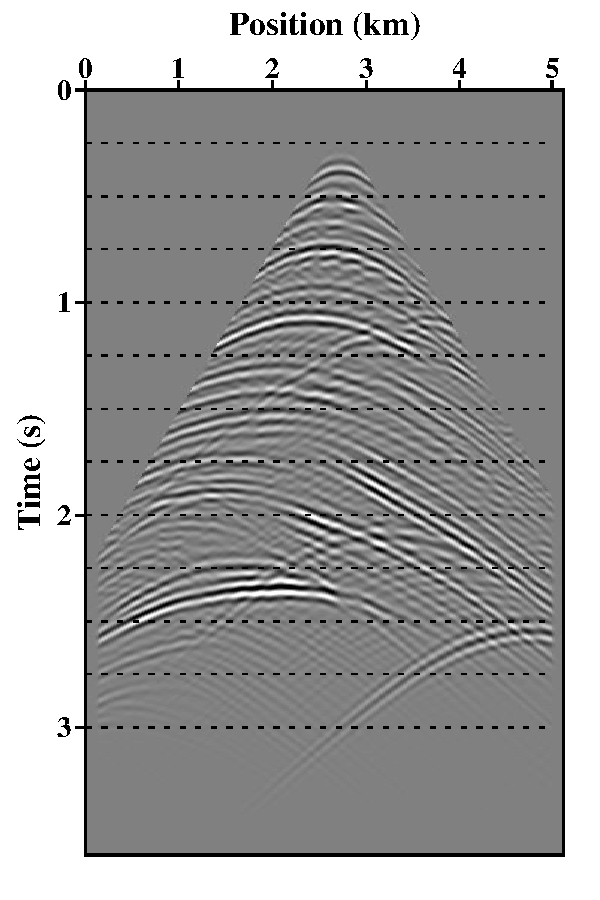
\includegraphics[width=0.33\textwidth]{Figure/chapter03/sigbee2/Fig/DataPP_werti.pdf}}\\
   \subfloat[]{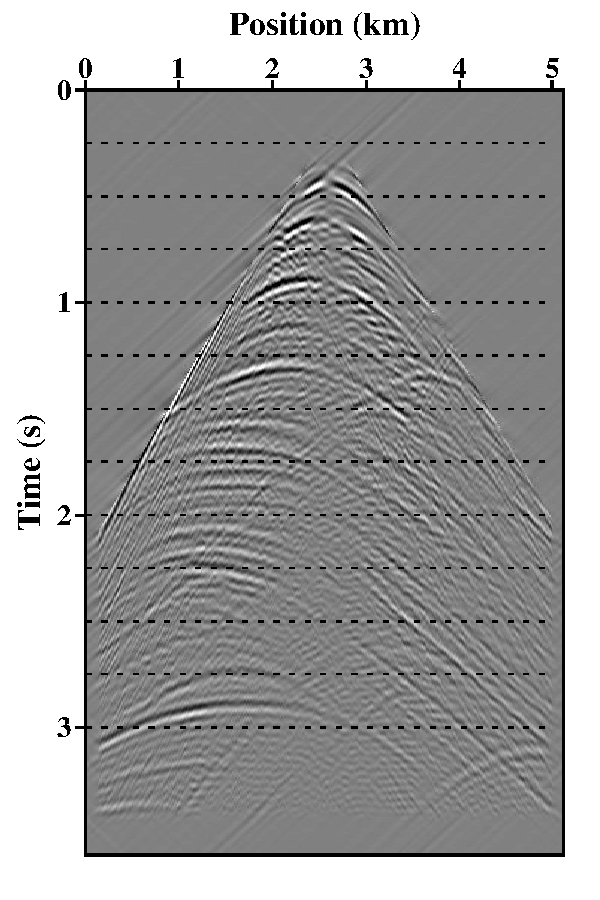
\includegraphics[width=0.33\textwidth]{Figure/chapter03/sigbee2/Fig/DataPS_true.pdf}}
   \subfloat[]{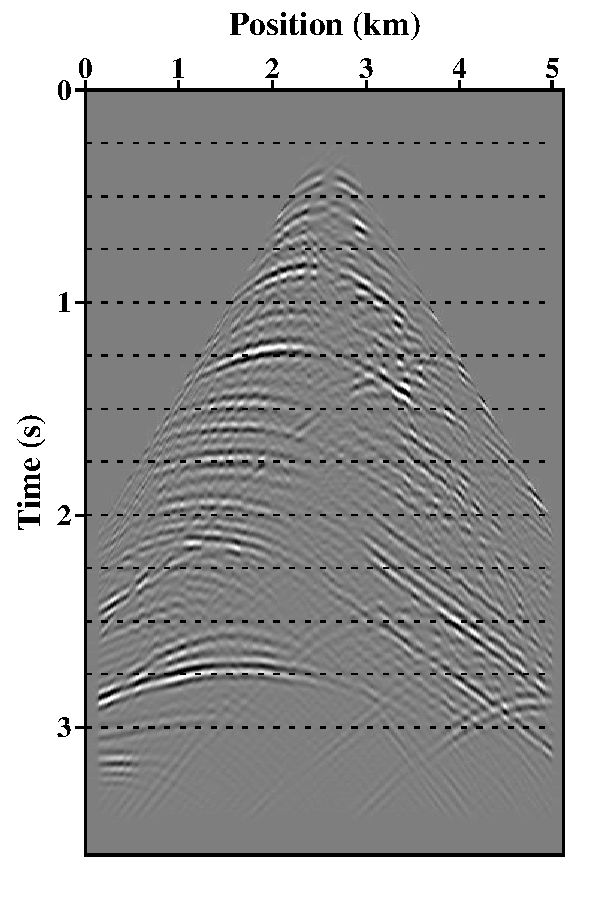
\includegraphics[width=0.33\textwidth]{Figure/chapter03/sigbee2/Fig/DataPS_init.pdf}}
   \subfloat[]{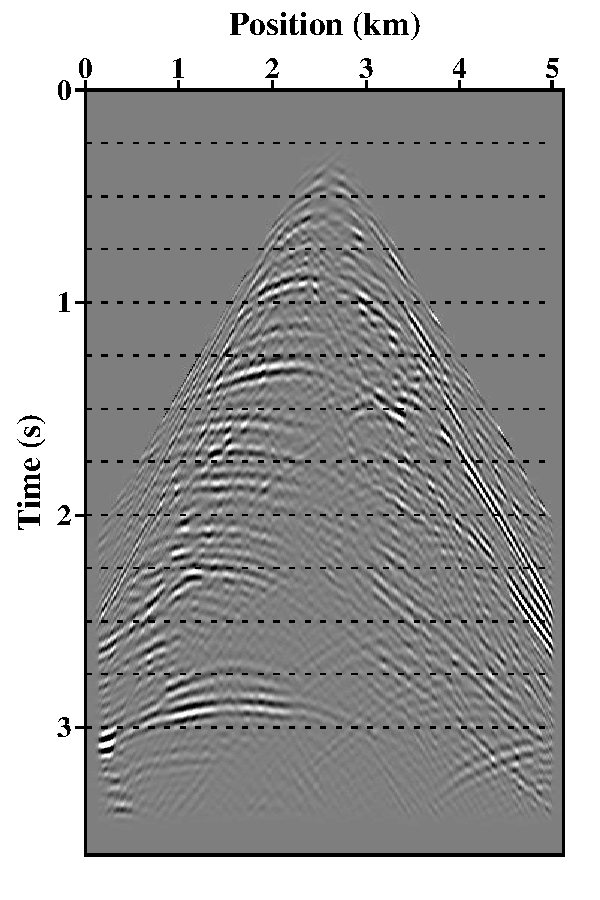
\includegraphics[width=0.33\textwidth]{Figure/chapter03/sigbee2/Fig/DataPS_werti.pdf}}
   \caption{真实反射数据(左),初始模型反偏移反射数据(中)与EWERTI之后反偏移反射数据(右)之间的比较:(a),(b)和(c)为垂直分量,(d),(e)和(f)为水平
   分量。}
   \label{fig:Data_comparison}
\end{figure}

采用上述模型重新进行ERTM成像,发现随着模型中深部波数成分的恢复,PP波与PS波的成像结果得到了很大的改善,绕射波也基本收敛。模型右侧
部分由于界面倾角以及观测孔径限制,反射波信息不足,EWERTI未能很好地恢复模型中低波数成分,成像结果不是十分聚焦。
此外,也将EWERTI前后模拟的反射数据与真实反射数据进行了对比。如图\ref{fig:Data_comparison}所示,可以看到经过EWERTI之后,主要反射同相轴
位置与真实数据已经相差无几。
如果采用该模型进行波形残差匹配,就不会出现cycle-skipping效应。因此在EWERTI之后考虑利用ERWI进一步恢复模型中低波数成分也未尝不可。
\begin{figure}[!htb]
   \centering
   \subfloat[]{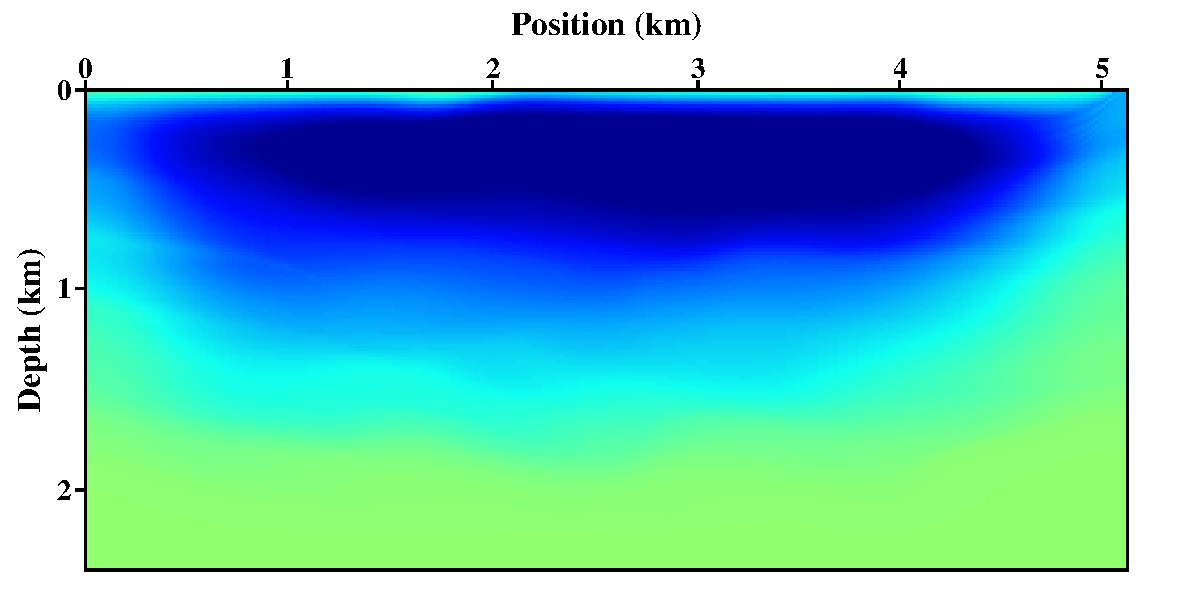
\includegraphics[width=0.5\textwidth]{Figure/chapter03/sigbee2/LSF_Gra_vp.pdf}}
   \subfloat[]{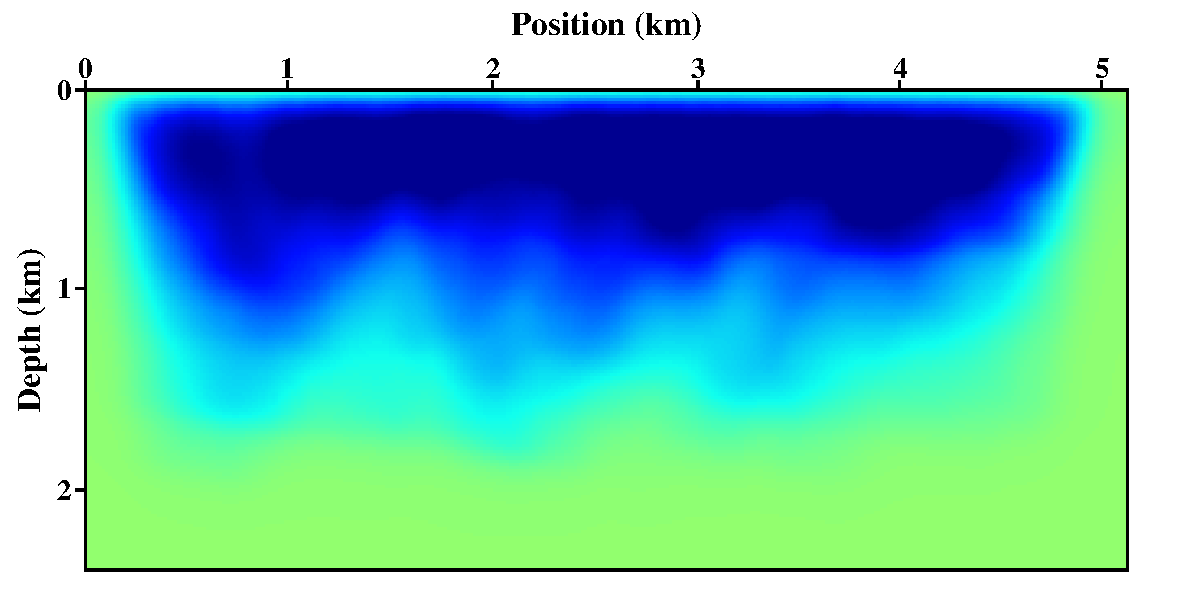
\includegraphics[width=0.5\textwidth]{Figure/chapter03/sigbee2/NoLSF_Gra_vp.pdf}}\\
   \subfloat[]{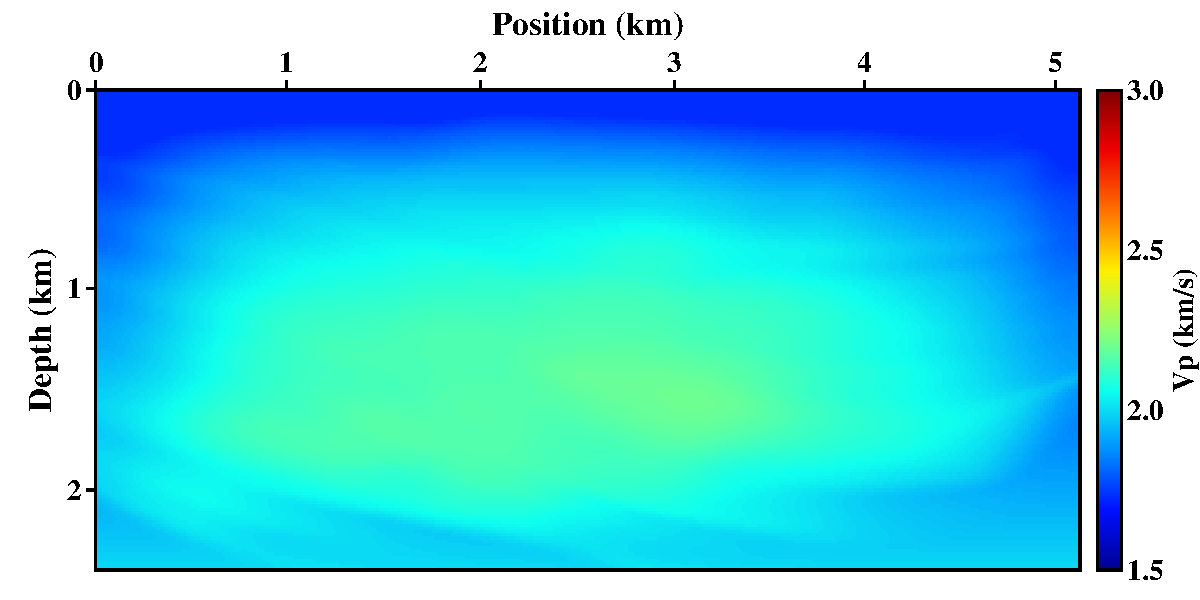
\includegraphics[width=0.5\textwidth]{Figure/chapter03/sigbee2/Fig/newinit3vp.pdf}}
   \subfloat[]{\includegraphics[width=0.5\textwidth]{Figure/chapter03/sigbee2/NoLSF_vp.pdf}}\\
   \caption{局部倾角滤波约束效果展示。(a)和(c)分别为倾角滤波约束下的首次迭代$V_p$梯度与最终反演结果,
   (b)和(d)分别为不加约束时首次迭代的$V_p$梯度与最终反演结果}
   \label{fig:LSF_comparison}
\end{figure}

\begin{figure}[!htb]
   \centering
   \subfloat[]{\includegraphics[width=0.5\textwidth]{Figure/chapter03/sigbee2/Fig/nodevp.pdf}}
   \subfloat[]{\includegraphics[width=0.5\textwidth]{Figure/chapter03/sigbee2/Fig/nodevs.pdf}}
   \caption{
	   采用EWERTI结果作为初始模型EFWI的反演结果。(a)为$V_p$, (b)为$V_s$。
%	   Inverted results of WERTI and EFWI. (a) and (b) are inverted $V_p$ and
%       $V_s$ model through two-stage elastic WERTI with the linearly increased models
%       as initial models. (c) and (d) are inverted $V_p$ and $V_s$ through EFWI using
%   (a) and (b) as starting models.
   }
   \label{fig:EWERTI+EFWI}
\end{figure}

局部倾角导引正则化对降低反演的多解性有着至关重要的作用。
在EWERTI过程中,每次迭代的梯度都采用该轮迭代中的ERTM图像来进行局部倾角约束滤波。从图\ref{fig:LSF_comparison}b中可以看到,
尽管EWERTI的梯度很光滑
,但是不加倾角约束滤波的梯度中包含了反射波的照明脚印,采用该梯度进行更新最后会得到图\ref{fig:LSF_comparison}d的反演结果,
将导致很难进一步地更新$V_s$模型。
而采用倾角约束滤波后,EWERTI获得了更加合理的反演结果,也为后续的$V_s$更新提供了较好的$V_p$初始模型。需要注意的是,虽然在$V_s$反演中,
采用PP波反射界面进行反偏移,但是仍然基于不断修正的PS波成像剖面进行局部倾角约束滤波对梯度进行平滑处理。
\begin{figure}[!htb]
   \centering
   \subfloat[]{\includegraphics[width=0.5\textwidth]{Figure/chapter03/sigbee2/Fig/1km.pdf}}
   \subfloat[]{\includegraphics[width=0.5\textwidth]{Figure/chapter03/sigbee2/Fig/3km.pdf}}
   \caption{
	   1.4km (a) 和3km (b) 处EWERTI和EFWI的垂向剖面对比。黑线和蓝线分别代表真实模型与初始模型,绿线与黄线分别代表WERTI和EFWI的结果。
%	   Vertical profiles of elastic WERTI and EFWI results at 1.4km (a) and
%       3km (b). The black and blue lines indicate the true and linearly increased
%       initial model. The green and yellow lines indicate the WERTI and EFWI results,
%       respectively.
   }
   \label{fig:Profiles}
\end{figure}

采用WERTI的反演结果作为初始模型,重新进行了
常规EFWI反演。这里EFWI的反演仍然采用从低频到高频的多尺度策略。在恢复了模型中低波数成分的情况下,EFWI不再受到cycle-skipping的
困扰。反演结果如图\ref{fig:EWERTI+EFWI}a和\ref{fig:EWERTI+EFWI}b所示,$V_p$和$V_s$模型的浅部以及
中深部都得到了很好的重建。但是模型右侧和底部中低波数分量未能很好的恢复,因此EFWI在此区域未能达到令人满意的反演效果,原因前文已经给出。
%在于地面观测下
%,模型右侧的反射波覆盖不够导致WERTI不能准确的恢复该区域速度的长波长分量。而且在模型最底部,由于缺乏反射波路径覆盖EWERTI并未起效
%,EFWI也最终无法恢复这部分的速度。
图\ref{fig:Profiles}也展示了1.4km和3km处
的“测井”曲线。从图中可以看出,
弹性WERTI能够提供可靠的包含长波长分量的初始模型,以此为基础的EFWI反演可以比较有效地恢复准确的弹性速度模型。

通常,cycle-skipping问题与数据中的低频以及初始模型中的中低波数成分密切相关。数据中有效的低频成分可以降低FWI对初始模型的依赖程度,
而较好地包含中低波数成分的初始模型则可以降低FWI对低频数据的依赖。实际数据处理中,由于低频分量中常常含有许多噪音干扰,使得FWI更依赖于良好
的初始模型。这里将进一步测试EWERTI+EFWI串级反演流程对数据中低频成分的依赖性。

采用图\ref{fig:InvertedModel_WERTI}中的结果作为初始模型,将分别从3Hz,5Hz和7Hz开始进行常规EFWI,
低于门槛值的频率成分将通过滤波切除,反演仍然遵循从低频到高频的多尺度策略,以观察EFWI在该初始模型下对数据中低频成分的依赖性。
实验结果如图\ref{fig:LowFreqCut_EFWI}所示,可见在滤掉3Hz以下的低频分量时,EFWI仍然可以获得较为满意的反演结果。左侧区域在截频达到7Hz的时候仍
能得到可以接受的反演结果。
但是随着低频门槛值的增大,
EFWI受到越来越严重的困扰,尤其是在EWERTI未能恢复中低波数的右侧区域。这表明,受观测孔径影响模型右侧比左侧更依赖数据中的低频信息。
%事实上在左侧区域,由于背景速度已经基本恢复准确,高频数据的EFWI反演已经接近于最小平方成像的过程。我们将在下一章对
%该问题做详细讨论。
\begin{figure}[!htb]
   \centering
   \subfloat[]{\includegraphics[width=0.5\textwidth]{Figure/chapter03/sigbee2/3Hzvp.pdf}}
   \subfloat[]{\includegraphics[width=0.5\textwidth]{Figure/chapter03/sigbee2/3Hzvs.pdf}}\\
   \subfloat[]{\includegraphics[width=0.5\textwidth]{Figure/chapter03/sigbee2/5Hzvp.pdf}}
   \subfloat[]{\includegraphics[width=0.5\textwidth]{Figure/chapter03/sigbee2/5Hzvs.pdf}}\\
   \subfloat[]{\includegraphics[width=0.5\textwidth]{Figure/chapter03/sigbee2/7Hzvp.pdf}}
   \subfloat[]{\includegraphics[width=0.5\textwidth]{Figure/chapter03/sigbee2/7Hzvs.pdf}}\\
   \caption{数据滤掉不同门槛的低频后EFWI的反演结果。(a), (c), (e)为$V_p$,(b), (d), (f)为$V_s$。
   第1,2,3行的低频截频分别为3Hz,5Hz和7Hz.}
   \label{fig:LowFreqCut_EFWI}
\end{figure}



\section{本章小结}
本章利用DIW拾取走时残差,将WERTI方法扩展到了弹性介质。由于模型的长波长成分与走时之间更趋于线性关系,
因此相对于采用波形拟合的目标函数,走时残差目标函数对规避cycle-skipping问题有着明显的优势,
可以更稳健地反演模型的长波长分量。相对空间或时间互相关提取走时残差的方法而言,DIW在模型复杂时更加稳健可靠。

针对弹性波场中复杂的模式转换问题,本文采用多分量地震数据的P/S分离技术分别获得PP与PS反射波数据,
进而提取模拟数据与观测数据之间的走时残差,采用空间波场模式解耦的方式来获得更具有物理含义的
PS反射波核函数来更新$V_s$模型。为了降低反演中的非线性程度,文中设计了两步法的策略,先反演$V_p$后反演$V_s$。通过局部倾角导引正则化约束,采用PP
波界面反偏移获取PS反射波,结合“层剥离”等手段来对反演进行控制,从而确保其收敛性。实验表明,本文EWERTI获得了较为可靠的包含中低波数成分的模型,为EFWI提供了良好的初始模型。
